% !TeX program = lualatex
% ================================================================
% Indonesian Parallel Text Version of Calendars
%
% Generated by the server using the following settings:
%
%   language            Indonesian (ind)
%   text direction      left to right
%   font                Noto Serif
%   fallback font       Noto Serif
%   built from          latex/worksheets/measures/time/calendars.tex
%   vocabulary key      latex/worksheets/measures/time/calendars/L2/ind/calendars_indonesianKey.tex
%   tier 3 vocabulary   green   RGB 0 128 0
%   English text        black   RGB 0 0 0
%   Indonesian text     purple  RGB 112 48 160
%   layout macros       version 3
%
% Please don't edit any information in this comment block - the server
% compares it against the current settings and rebuilds this file when
% they differ, so changes here would be overwritten. However, feel free
% to make updates to the LaTeX below if you want to edit it.
% ================================================================

\documentclass[11pt,a4paper]{article}
% ================================================================
% Copied from the English sheet this was translated from, so that
% anything it sets up for itself still works here
% ================================================================
\usepackage[margin=1.25cm, top=1.1cm, bottom=1.2cm]{geometry}
\usepackage[scaled]{helvet}\renewcommand\familydefault{\sfdefault}
\usepackage[T1]{fontenc}
\usepackage{tikz,xcolor,array,tabularx,booktabs,enumitem,multicol}
\usetikzlibrary{arrows.meta,shapes.misc,calc}
\pagestyle{empty}\setlength{\parindent}{0pt}
\definecolor{ttdark}{HTML}{2B2D5C}
\definecolor{ttaccent}{HTML}{D9480F}
\definecolor{ttglow}{HTML}{25B5A4}
\definecolor{ttpale}{HTML}{EEF1FA}
\tikzset{flag/.style={draw=ttaccent, fill=white, text=ttaccent, line width=0.8pt, font=\tiny\bfseries, rounded corners=2pt, inner sep=2pt, align=center}}
\newcommand{\banner}[1]{{\color{ttdark}\large\bfseries #1}\par\vspace{-7pt}{\color{ttdark}\rule{\linewidth}{1.2pt}}\par\vspace{-2pt}}
% time machine dial: \dial{BACK|FORWARD}{amount}{unit}
\newcommand{\dial}[3]{\tikz[baseline=-3.5pt]{\node[draw=ttdark, line width=1pt, rounded corners=3pt, inner sep=1.5pt] {%
  \tikz[baseline]{\node[draw=black!45, text=ttdark, font=\scriptsize\bfseries, inner sep=2.5pt, minimum width=1.5cm]{#1};}\,%
  \tikz[baseline]{\node[draw=black!45, text=black, font=\scriptsize\bfseries, inner sep=2.5pt, minimum width=1.3cm]{#2};}\,%
  \tikz[baseline]{\node[draw=black!45, text=ttdark, font=\scriptsize\bfseries, inner sep=2.5pt, minimum width=1.6cm]{#3};}};}}
\newcommand{\aline}{\rule{2.6cm}{0.4pt}}
\newcommand{\lline}{\rule{4.6cm}{0.4pt}}
\newcommand{\ans}[1]{\textcolor{red!75!black}{\bfseries #1}}
\newcommand{\factbox}[2]{\begin{tikzpicture}\node[draw=ttdark, rounded corners=4pt, line width=1pt, inner sep=7pt, text width=#1, align=left, font=\small]{#2};\end{tikzpicture}}

% Characters this language's font has not got are borrowed from another,
% rather than being silently dropped - see docs/translated-sheet-latex.md
\directlua{%
  if luaotfload and luaotfload.add_fallback then
    luaotfload.add_fallback("eallatinfallback",
      { "Noto Serif:mode=harf;" })
  else
    tex.error("this luaotfload is too old to register a fallback font")
  end
}
\usepackage[english]{babel}
\babelprovide[import]{indonesian}
\babelfont[indonesian]{rm}[Renderer=Harfbuzz, BoldFont={Noto Serif}, ItalicFont={Noto Serif}, BoldItalicFont={Noto Serif}, RawFeature={fallback=eallatinfallback}]{Noto Serif}
\babelfont[indonesian]{sf}[Renderer=Harfbuzz, BoldFont={Noto Serif}, ItalicFont={Noto Serif}, BoldItalicFont={Noto Serif}, RawFeature={fallback=eallatinfallback}]{Noto Serif}
\newcommand{\ealtext}[1]{\foreignlanguage{indonesian}{#1}}
\newcommand{\ealtextblock}[1]{{\raggedright\foreignlanguage{indonesian}{#1}\par}}
% ================================================================
% EAL layout helpers
% ================================================================
\usepackage{xcolor}

\definecolor{ealkeycolour}{RGB}{0,128,0}
\definecolor{ealenglish}{RGB}{0,0,0}
\definecolor{ealtwocolour}{RGB}{112,48,160}

\newsavebox{\ealboxen}
\newsavebox{\ealboxtr}
\newlength{\ealglosswd}
\newlength{\ealglossraise}
\setlength{\ealglossraise}{1.15em}

% a tier 3 word, in English and in translation alike
\newcommand{\ealkey}[1]{\textcolor{ealkeycolour}{#1}}
\newcommand{\ealkeytr}[1]{\textcolor{ealkeycolour}{\ealtext{#1}}}

% One translated word above one English word. Built from kernel
% primitives, never a tabular, which would break wherever the sheet
% loads array, booktabs or tabularx. The box is as wide as the wider of
% the two, so a long translation pushes its neighbours aside instead of
% overlapping them, and it claims its full height so a table row or a
% TikZ node makes room for it.
\newcommand{\ealgloss}[2]{%
  \sbox{\ealboxen}{\ealkey{#1}}%
  \sbox{\ealboxtr}{\small\textcolor{ealtwocolour}{\ealtext{#2}}}%
  \setlength{\ealglosswd}{\wd\ealboxen}%
  \ifdim\wd\ealboxtr>\ealglosswd\setlength{\ealglosswd}{\wd\ealboxtr}\fi
  \leavevmode
  \makebox[\ealglosswd][c]{%
    \makebox[0pt][c]{\usebox{\ealboxen}}%
    \makebox[0pt][c]{\raisebox{\ealglossraise}{\usebox{\ealboxtr}}}%
  }%
}

% opens up line spacing around a block of glosses, so the raised
% translations sit clear of the line above
\newenvironment{ealglossed}{\par\linespread{2.1}\selectfont\ignorespaces}{\par}

% a whole translated sentence above its English counterpart. block level,
% so it does not belong inside a tabular cell
\newcommand{\ealpara}[2]{%
  \par\addvspace{0.5\baselineskip}%
  {\color{ealtwocolour}\ealtextblock{#1}}%
  \penalty200
  {\color{ealenglish}#2\par}%
  \addvspace{0.5\baselineskip}%
}

\begin{document}

\ealpara{Penjelajah Waktu!}{Time Travellers!}
\ealpara{\ealkeytr{Kalender}, \ealkeytr{konversi} dan \ealkeytr{garis waktu}}{Calendars, \ealkey{conversions} and \ealkey{timelines}}


\begin{tikzpicture}
\node[draw=ttdark, line width=1.5pt, rounded corners=6pt, minimum width=\linewidth, minimum height=1.9cm] (h) {};
\node[text=ttdark, font=\fontsize{30}{32}\selectfont\bfseries, anchor=west] at ($(h.west)+(0.5,0.18)$) {Time Travellers!};
\node[text=ttaccent, font=\small\bfseries, anchor=west] at ($(h.west)+(0.55,-0.6)$) {Calendars, conversions and timelines};
\begin{scope}[shift={($(h.east)+(-1.4,0)$)}]
\draw[ttdark, line width=1.5pt] (0,0) circle (0.72); \foreach \a in {0,30,...,330} \draw[ttdark] (\a:0.58) -- (\a:0.72);
\draw[ttdark, line width=2pt, -{Stealth[length=4pt]}] (0,0) -- (115:0.42); \draw[ttdark, line width=1.2pt, -{Stealth[length=4pt]}] (0,0) -- (-160:0.6);
\draw[ttaccent, line width=1.8pt, -{Stealth[length=6pt]}] (40:0.95) arc (40:-200:0.95);
\end{scope}
\end{tikzpicture}\par\medskip

\ealpara{Bagian A \quad Lompatan \ealkeytr{kalender} --- lompatan kecil}{}
\banner{Part A \quad \ealkey{Calendar} hops --- small jumps}\par\smallskip

\ealpara{Mesin waktu Dr Chrono diparkir di tempat parkir sekolah. \textbf{Sekarang hari Sabtu, 31 Oktober 2026, pukul 10.00} (dilingkari). Untuk setiap pengaturan dial, gunakan \ealkeytr{kalender} untuk menemukan di mana mesin mendarat jika Dr Chrono bepergian dari Sabtu, 31 Oktober 2026, pukul 10.00.}{Dr Chrono's time machine is parked in the school car park. \textbf{It is Saturday 31 October 2026, 10:00} (circled). For each dial setting, use the \ealkey{calendars} to find where the machine lands if Dr Chrono travels from Saturday 31 October 2026, 10:00.}\par\medskip

\begin{center}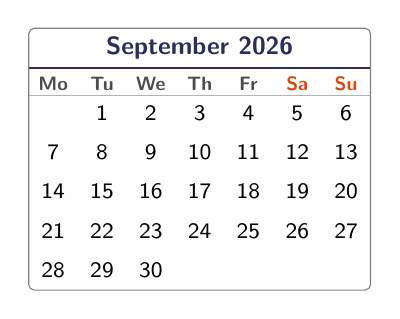
\begin{tikzpicture}[x=0.62cm,y=0.50cm,baseline=(current bounding box.north)]
\node[text=ttdark, font=\bfseries\small] at (3.5,0.65) {September 2026}; \draw[ttdark, thick] (0,0.15) -- (7,0.15);
\node[font=\scriptsize\bfseries, text=black!70] at (0.5,-0.25) {Mo};
\node[font=\scriptsize\bfseries, text=black!70] at (1.5,-0.25) {Tu};
\node[font=\scriptsize\bfseries, text=black!70] at (2.5,-0.25) {We};
\node[font=\scriptsize\bfseries, text=black!70] at (3.5,-0.25) {Th};
\node[font=\scriptsize\bfseries, text=black!70] at (4.5,-0.25) {Fr};
\node[font=\scriptsize\bfseries, text=ttaccent] at (5.5,-0.25) {Sa};
\node[font=\scriptsize\bfseries, text=ttaccent] at (6.5,-0.25) {Su};
\node[font=\footnotesize] at (1.5,-1.0) {1};
\node[font=\footnotesize] at (2.5,-1.0) {2};
\node[font=\footnotesize] at (3.5,-1.0) {3};
\node[font=\footnotesize] at (4.5,-1.0) {4};
\node[font=\footnotesize] at (5.5,-1.0) {5};
\node[font=\footnotesize] at (6.5,-1.0) {6};
\node[font=\footnotesize] at (0.5,-2.0) {7};
\node[font=\footnotesize] at (1.5,-2.0) {8};
\node[font=\footnotesize] at (2.5,-2.0) {9};
\node[font=\footnotesize] at (3.5,-2.0) {10};
\node[font=\footnotesize] at (4.5,-2.0) {11};
\node[font=\footnotesize] at (5.5,-2.0) {12};
\node[font=\footnotesize] at (6.5,-2.0) {13};
\node[font=\footnotesize] at (0.5,-3.0) {14};
\node[font=\footnotesize] at (1.5,-3.0) {15};
\node[font=\footnotesize] at (2.5,-3.0) {16};
\node[font=\footnotesize] at (3.5,-3.0) {17};
\node[font=\footnotesize] at (4.5,-3.0) {18};
\node[font=\footnotesize] at (5.5,-3.0) {19};
\node[font=\footnotesize] at (6.5,-3.0) {20};
\node[font=\footnotesize] at (0.5,-4.0) {21};
\node[font=\footnotesize] at (1.5,-4.0) {22};
\node[font=\footnotesize] at (2.5,-4.0) {23};
\node[font=\footnotesize] at (3.5,-4.0) {24};
\node[font=\footnotesize] at (4.5,-4.0) {25};
\node[font=\footnotesize] at (5.5,-4.0) {26};
\node[font=\footnotesize] at (6.5,-4.0) {27};
\node[font=\footnotesize] at (0.5,-5.0) {28};
\node[font=\footnotesize] at (1.5,-5.0) {29};
\node[font=\footnotesize] at (2.5,-5.0) {30};
\draw[black!30] (0,-0.55) -- (7,-0.55);
\draw[black!50, rounded corners=2pt] (0,-5.5) rectangle (7,1.15);
\end{tikzpicture}\hfill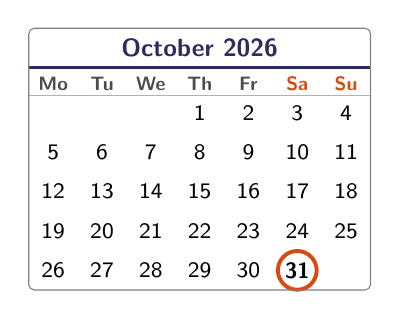
\begin{tikzpicture}[x=0.62cm,y=0.50cm,baseline=(current bounding box.north)]
\node[text=ttdark, font=\bfseries\small] at (3.5,0.65) {October 2026}; \draw[ttdark, thick] (0,0.15) -- (7,0.15);
\node[font=\scriptsize\bfseries, text=black!70] at (0.5,-0.25) {Mo};
\node[font=\scriptsize\bfseries, text=black!70] at (1.5,-0.25) {Tu};
\node[font=\scriptsize\bfseries, text=black!70] at (2.5,-0.25) {We};
\node[font=\scriptsize\bfseries, text=black!70] at (3.5,-0.25) {Th};
\node[font=\scriptsize\bfseries, text=black!70] at (4.5,-0.25) {Fr};
\node[font=\scriptsize\bfseries, text=ttaccent] at (5.5,-0.25) {Sa};
\node[font=\scriptsize\bfseries, text=ttaccent] at (6.5,-0.25) {Su};
\node[font=\footnotesize] at (3.5,-1.0) {1};
\node[font=\footnotesize] at (4.5,-1.0) {2};
\node[font=\footnotesize] at (5.5,-1.0) {3};
\node[font=\footnotesize] at (6.5,-1.0) {4};
\node[font=\footnotesize] at (0.5,-2.0) {5};
\node[font=\footnotesize] at (1.5,-2.0) {6};
\node[font=\footnotesize] at (2.5,-2.0) {7};
\node[font=\footnotesize] at (3.5,-2.0) {8};
\node[font=\footnotesize] at (4.5,-2.0) {9};
\node[font=\footnotesize] at (5.5,-2.0) {10};
\node[font=\footnotesize] at (6.5,-2.0) {11};
\node[font=\footnotesize] at (0.5,-3.0) {12};
\node[font=\footnotesize] at (1.5,-3.0) {13};
\node[font=\footnotesize] at (2.5,-3.0) {14};
\node[font=\footnotesize] at (3.5,-3.0) {15};
\node[font=\footnotesize] at (4.5,-3.0) {16};
\node[font=\footnotesize] at (5.5,-3.0) {17};
\node[font=\footnotesize] at (6.5,-3.0) {18};
\node[font=\footnotesize] at (0.5,-4.0) {19};
\node[font=\footnotesize] at (1.5,-4.0) {20};
\node[font=\footnotesize] at (2.5,-4.0) {21};
\node[font=\footnotesize] at (3.5,-4.0) {22};
\node[font=\footnotesize] at (4.5,-4.0) {23};
\node[font=\footnotesize] at (5.5,-4.0) {24};
\node[font=\footnotesize] at (6.5,-4.0) {25};
\node[font=\footnotesize] at (0.5,-5.0) {26};
\node[font=\footnotesize] at (1.5,-5.0) {27};
\node[font=\footnotesize] at (2.5,-5.0) {28};
\node[font=\footnotesize] at (3.5,-5.0) {29};
\node[font=\footnotesize] at (4.5,-5.0) {30};
\node[circle, draw=ttaccent, line width=1.4pt, inner sep=0pt, minimum size=14pt] at (5.5,-5.0) {};
\node[font=\footnotesize\bfseries, text=black] at (5.5,-5.0) {31};
\draw[black!30] (0,-0.55) -- (7,-0.55);
\draw[black!50, rounded corners=2pt] (0,-5.5) rectangle (7,1.15);
\end{tikzpicture}\hfill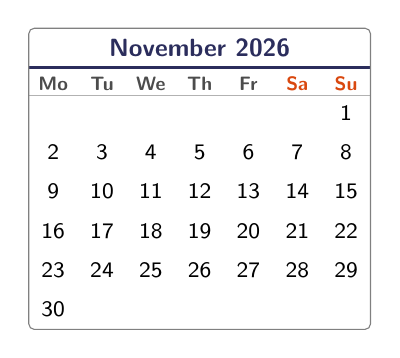
\begin{tikzpicture}[x=0.62cm,y=0.50cm,baseline=(current bounding box.north)]
\node[text=ttdark, font=\bfseries\small] at (3.5,0.65) {November 2026}; \draw[ttdark, thick] (0,0.15) -- (7,0.15);
\node[font=\scriptsize\bfseries, text=black!70] at (0.5,-0.25) {Mo};
\node[font=\scriptsize\bfseries, text=black!70] at (1.5,-0.25) {Tu};
\node[font=\scriptsize\bfseries, text=black!70] at (2.5,-0.25) {We};
\node[font=\scriptsize\bfseries, text=black!70] at (3.5,-0.25) {Th};
\node[font=\scriptsize\bfseries, text=black!70] at (4.5,-0.25) {Fr};
\node[font=\scriptsize\bfseries, text=ttaccent] at (5.5,-0.25) {Sa};
\node[font=\scriptsize\bfseries, text=ttaccent] at (6.5,-0.25) {Su};
\node[font=\footnotesize] at (6.5,-1.0) {1};
\node[font=\footnotesize] at (0.5,-2.0) {2};
\node[font=\footnotesize] at (1.5,-2.0) {3};
\node[font=\footnotesize] at (2.5,-2.0) {4};
\node[font=\footnotesize] at (3.5,-2.0) {5};
\node[font=\footnotesize] at (4.5,-2.0) {6};
\node[font=\footnotesize] at (5.5,-2.0) {7};
\node[font=\footnotesize] at (6.5,-2.0) {8};
\node[font=\footnotesize] at (0.5,-3.0) {9};
\node[font=\footnotesize] at (1.5,-3.0) {10};
\node[font=\footnotesize] at (2.5,-3.0) {11};
\node[font=\footnotesize] at (3.5,-3.0) {12};
\node[font=\footnotesize] at (4.5,-3.0) {13};
\node[font=\footnotesize] at (5.5,-3.0) {14};
\node[font=\footnotesize] at (6.5,-3.0) {15};
\node[font=\footnotesize] at (0.5,-4.0) {16};
\node[font=\footnotesize] at (1.5,-4.0) {17};
\node[font=\footnotesize] at (2.5,-4.0) {18};
\node[font=\footnotesize] at (3.5,-4.0) {19};
\node[font=\footnotesize] at (4.5,-4.0) {20};
\node[font=\footnotesize] at (5.5,-4.0) {21};
\node[font=\footnotesize] at (6.5,-4.0) {22};
\node[font=\footnotesize] at (0.5,-5.0) {23};
\node[font=\footnotesize] at (1.5,-5.0) {24};
\node[font=\footnotesize] at (2.5,-5.0) {25};
\node[font=\footnotesize] at (3.5,-5.0) {26};
\node[font=\footnotesize] at (4.5,-5.0) {27};
\node[font=\footnotesize] at (5.5,-5.0) {28};
\node[font=\footnotesize] at (6.5,-5.0) {29};
\node[font=\footnotesize] at (0.5,-6.0) {30};
\draw[black!30] (0,-0.55) -- (7,-0.55);
\draw[black!50, rounded corners=2pt] (0,-6.5) rectangle (7,1.15);
\end{tikzpicture}\hfill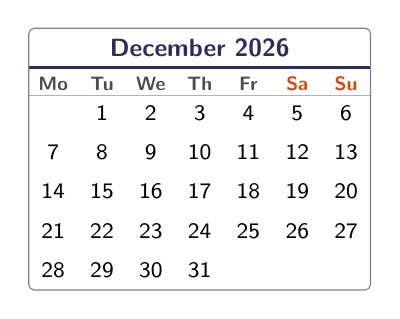
\begin{tikzpicture}[x=0.62cm,y=0.50cm,baseline=(current bounding box.north)]
\node[text=ttdark, font=\bfseries\small] at (3.5,0.65) {December 2026}; \draw[ttdark, thick] (0,0.15) -- (7,0.15);
\node[font=\scriptsize\bfseries, text=black!70] at (0.5,-0.25) {Mo};
\node[font=\scriptsize\bfseries, text=black!70] at (1.5,-0.25) {Tu};
\node[font=\scriptsize\bfseries, text=black!70] at (2.5,-0.25) {We};
\node[font=\scriptsize\bfseries, text=black!70] at (3.5,-0.25) {Th};
\node[font=\scriptsize\bfseries, text=black!70] at (4.5,-0.25) {Fr};
\node[font=\scriptsize\bfseries, text=ttaccent] at (5.5,-0.25) {Sa};
\node[font=\scriptsize\bfseries, text=ttaccent] at (6.5,-0.25) {Su};
\node[font=\footnotesize] at (1.5,-1.0) {1};
\node[font=\footnotesize] at (2.5,-1.0) {2};
\node[font=\footnotesize] at (3.5,-1.0) {3};
\node[font=\footnotesize] at (4.5,-1.0) {4};
\node[font=\footnotesize] at (5.5,-1.0) {5};
\node[font=\footnotesize] at (6.5,-1.0) {6};
\node[font=\footnotesize] at (0.5,-2.0) {7};
\node[font=\footnotesize] at (1.5,-2.0) {8};
\node[font=\footnotesize] at (2.5,-2.0) {9};
\node[font=\footnotesize] at (3.5,-2.0) {10};
\node[font=\footnotesize] at (4.5,-2.0) {11};
\node[font=\footnotesize] at (5.5,-2.0) {12};
\node[font=\footnotesize] at (6.5,-2.0) {13};
\node[font=\footnotesize] at (0.5,-3.0) {14};
\node[font=\footnotesize] at (1.5,-3.0) {15};
\node[font=\footnotesize] at (2.5,-3.0) {16};
\node[font=\footnotesize] at (3.5,-3.0) {17};
\node[font=\footnotesize] at (4.5,-3.0) {18};
\node[font=\footnotesize] at (5.5,-3.0) {19};
\node[font=\footnotesize] at (6.5,-3.0) {20};
\node[font=\footnotesize] at (0.5,-4.0) {21};
\node[font=\footnotesize] at (1.5,-4.0) {22};
\node[font=\footnotesize] at (2.5,-4.0) {23};
\node[font=\footnotesize] at (3.5,-4.0) {24};
\node[font=\footnotesize] at (4.5,-4.0) {25};
\node[font=\footnotesize] at (5.5,-4.0) {26};
\node[font=\footnotesize] at (6.5,-4.0) {27};
\node[font=\footnotesize] at (0.5,-5.0) {28};
\node[font=\footnotesize] at (1.5,-5.0) {29};
\node[font=\footnotesize] at (2.5,-5.0) {30};
\node[font=\footnotesize] at (3.5,-5.0) {31};
\draw[black!30] (0,-0.55) -- (7,-0.55);
\draw[black!50, rounded corners=2pt] (0,-5.5) rectangle (7,1.15);
\end{tikzpicture}\end{center}\vspace{-2pt}

{\small \begin{enumerate}[label=\textbf{\arabic*.}, leftmargin=*, itemsep=5pt, topsep=4pt, start=1]
\item \ealpara{\dial{FORWARD}{1}{WEEK} \quad Hari dan tanggal: \lline}{\dial{FORWARD}{1}{WEEK} \quad Day and date: \lline}
\item \ealpara{\dial{FORWARD}{10}{DAYS} \quad Hari dan tanggal: \lline}{\dial{FORWARD}{10}{DAYS} \quad Day and date: \lline}
\item \ealpara{\dial{BACK}{2}{WEEKS} \quad Hari dan tanggal: \lline}{\dial{BACK}{2}{WEEKS} \quad Day and date: \lline}
\item \ealpara{\dial{FORWARD}{3 WEEKS}{+ 2 DAYS} \quad Hari dan tanggal: \lline}{\dial{FORWARD}{3 WEEKS}{+ 2 DAYS} \quad Day and date: \lline}
\item \ealpara{\dial{BACK}{45}{DAYS} \quad Hari dan tanggal: \lline}{\dial{BACK}{45}{DAYS} \quad Day and date: \lline}
\item \ealpara{\dial{FORWARD}{100}{HOURS} \quad Hari, tanggal \emph{dan waktu}: \lline}{\dial{FORWARD}{100}{HOURS} \quad Day, date \emph{and time}: \lline}
\item \ealpara{Dr Chrono ingin menonton kembang api pada Malam Bonfire (5 November) lalu melompat ke Hari Natal (25 Desember). Berapa hari ke depan itu? \aline\ \ Tulis dalam minggu dan hari: \aline}{Dr Chrono wants to watch the fireworks on Bonfire Night (5 November) and then jump to Christmas Day (25 December). How many days forward is that? \aline\ \ Write it in weeks and days: \aline}
\item \ealpara{Dial macet sehingga hanya bisa melompat dalam \textbf{minggu utuh}. Mulai dari hari ini, dapatkah Dr Chrono mendarat tepat pada Hari Natal? Jelaskan, dan sebutkan dua tanggal terdekat Natal yang \emph{dapat} dicapai.}{The dial gets stuck so it can only jump in \textbf{whole weeks}. Starting from today, can Dr Chrono land exactly on Christmas Day? Explain, and say which two dates nearest Christmas it \emph{can} reach.}\par\vspace{4pt}\rule{\linewidth}{0.4pt}
\item \ealpara{\textbf{Pendaratan seram:} Mesin Dr Chrono selalu rusak pada hari Jumat tanggal 13. Tanggal mana pada \ealkeytr{kalender} ini yang harus dia hindari? \lline}{\textbf{Spooky landing:} Dr Chrono's machine always breaks down on a Friday the 13th. Which date on these \ealkey{calendars} should she avoid? \lline}
\end{enumerate}}

\clearpage

\ealpara{Bagian B \quad Stasiun \ealkeytr{konversi} --- lompatan sedang}{}
\banner{Part B \quad \ealkey{Conversion} station --- medium jumps}\par\smallskip

\ealpara{Dial mesin waktu terkadang menunjukkan lompatan dalam \ealkeytr{satuan} yang aneh. Gunakan tangga \ealkeytr{konversi} untuk mengubahnya menjadi \ealkeytr{satuan} yang masuk akal.}{The time machine's dial sometimes shows jumps in strange \ealkey{units}. Use the \ealkey{conversion} ladder to change them into \ealkey{units} that make sense.}\par\medskip

\ealpara{\textbf{Tahun kabisat}\\ Satu tahun normal memiliki 365 hari. Satu \textbf{tahun kabisat} memiliki 366 hari (ada 29 Februari).\\[3pt]Tahun kabisat \ealkeytr{habis dibagi} 4 \ldots\ \emph{kecuali} \ealkeytr{tahun abad} (seperti 1900), yang harus \ealkeytr{habis dibagi} 400.}{}

\noindent\begin{minipage}[c]{0.66\linewidth}\centering 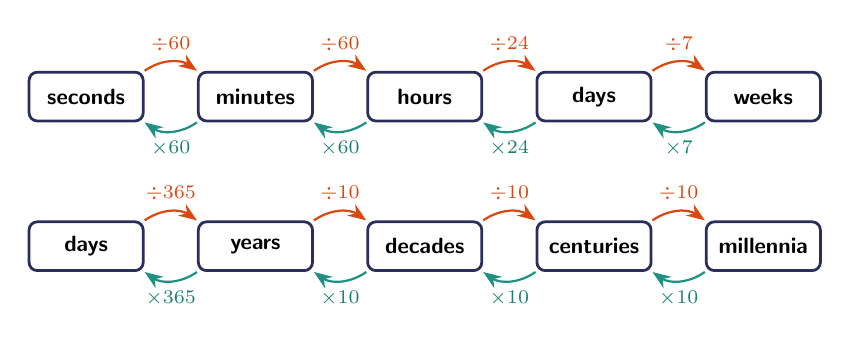
\begin{tikzpicture}[box/.style={draw=ttdark, fill=white, rounded corners=3pt, line width=1pt, minimum width=1.45cm, minimum height=0.62cm, font=\footnotesize\bfseries},
  up/.style={-{Stealth}, ttaccent, thick}, lab/.style={font=\scriptsize, text=ttaccent}]
\foreach \n/\x in {seconds/0, minutes/2.15, hours/4.3, days/6.45, weeks/8.6} \node[box] (\n) at (\x,0) {\n};
\foreach \a/\b/\k in {seconds/minutes/60, minutes/hours/60, hours/days/24, days/weeks/7}{
  \draw[up] ($(\a.north east)+(0,0)$) to[bend left=35] node[above, lab]{$\div\k$} ($(\b.north west)$);
  \draw[up, ttglow!80!black] ($(\b.south west)$) to[bend left=35] node[below, lab, text=ttglow!70!black]{$\times\k$} ($(\a.south east)$);}
\foreach \n/\x in {days/0, years/2.15, decades/4.3, centuries/6.45, millennia/8.6} \node[box] (\n2) at (\x,-1.9) {\n};
\foreach \a/\b/\k in {days/years/365, years/decades/10, decades/centuries/10, centuries/millennia/10}{
  \draw[up] ($(\a2.north east)$) to[bend left=35] node[above, lab]{$\div\k$} ($(\b2.north west)$);
  \draw[up, ttglow!80!black] ($(\b2.south west)$) to[bend left=35] node[below, lab, text=ttglow!70!black]{$\times\k$} ($(\a2.south east)$);}
\end{tikzpicture}\end{minipage}\hfill\begin{minipage}[c]{0.32\linewidth}\factbox{5.4cm}{\textbf{\ealkey{Leap years}}\\ A normal year has 365 days. A \textbf{\ealkey{leap year}} has 366 (it has 29 February).\\[3pt]\ealkey{Leap years} are \ealkey{divisible} by 4 \ldots\ \emph{except} \ealkey{century years} (like 1900), which must be \ealkey{divisible} by 400.}\end{minipage}\par\medskip

\ealpara{\textbf{1.} Ubah: 3 minggu = \rule{1.6cm}{0.4pt} hari; 4 \ealkeytr{abad} = \rule{1.6cm}{0.4pt} \ealkeytr{dekade}; 2 hari = \rule{1.6cm}{0.4pt} jam; 2 \ealkeytr{milenium} = \rule{1.6cm}{0.4pt} \ealkeytr{abad}; 180 menit = \rule{1.6cm}{0.4pt} jam; 7200 detik = \rule{1.6cm}{0.4pt} jam; 5 \ealkeytr{dekade} = \rule{1.6cm}{0.4pt} tahun; 3 hari = \rule{1.6cm}{0.4pt} menit}{\textbf{1.}\ Convert: 3 weeks = \rule{1.6cm}{0.4pt} days; 4 \ealkey{centuries} = \rule{1.6cm}{0.4pt} \ealkey{decades}; 2 days = \rule{1.6cm}{0.4pt} hours; 2 \ealkey{millennia} = \rule{1.6cm}{0.4pt} \ealkey{centuries}; 180 minutes = \rule{1.6cm}{0.4pt} hours; 7200 seconds = \rule{1.6cm}{0.4pt} hours; 5 \ealkey{decades} = \rule{1.6cm}{0.4pt} years; 3 days = \rule{1.6cm}{0.4pt} minutes}

{\small\begin{tabular}{rclp{1.6cm}p{0.6cm}rcll}3 weeks & = & \rule{1.6cm}{0.4pt} & days && 4 \ealkey{centuries} & = & \rule{1.6cm}{0.4pt} & \ealkey{decades}\\[4pt]
2 days & = & \rule{1.6cm}{0.4pt} & hours && 2 \ealkey{millennia} & = & \rule{1.6cm}{0.4pt} & \ealkey{centuries}\\[4pt]
180 minutes & = & \rule{1.6cm}{0.4pt} & hours && 7200 seconds & = & \rule{1.6cm}{0.4pt} & hours\\[4pt]
5 \ealkey{decades} & = & \rule{1.6cm}{0.4pt} & years && 3 days & = & \rule{1.6cm}{0.4pt} & minutes\\[4pt]\end{tabular}}\par\medskip

{\small \begin{enumerate}[label=\textbf{\arabic*.}, leftmargin=*, itemsep=5pt, topsep=4pt, start=2]
\item \ealpara{Tulis setiap bacaan dial dengan cara yang lebih masuk akal.}{Write each dial reading in a more sensible way.}
\ealpara{\dial{FORWARD}{72}{HOURS} = \rule{3.5cm}{0.4pt} hari; \dial{FORWARD}{420}{DAYS} = \rule{3.5cm}{0.4pt} minggu; \dial{BACK}{1000}{HOURS} = \rule{1.5cm}{0.4pt} hari dan \rule{1.5cm}{0.4pt} jam; \dial{BACK}{1000000}{SECONDS} \textbf{Tantangan:} = \rule{0.8cm}{0.4pt} h \rule{0.8cm}{0.4pt} j \rule{0.8cm}{0.4pt} mnt \rule{0.8cm}{0.4pt} dtk}{}
\begin{tabular}{@{}ll}\dial{FORWARD}{72}{HOURS} & = \rule{3.5cm}{0.4pt} days\\[5pt]\dial{FORWARD}{420}{DAYS} & = \rule{3.5cm}{0.4pt} weeks\\[5pt]\dial{BACK}{1000}{HOURS} & = \rule{1.5cm}{0.4pt} days and \rule{1.5cm}{0.4pt} hours\\[5pt]\dial{BACK}{1000000}{SECONDS} & \textbf{Challenge:} = \rule{0.8cm}{0.4pt} d \rule{0.8cm}{0.4pt} h \rule{0.8cm}{0.4pt} min \rule{0.8cm}{0.4pt} s\end{tabular}
\item \ealpara{Dr Chrono mendarat pada \textbf{29 Februari}. Tahun mana saja berikut yang mungkin? Lingkari: \quad 2028 \quad 2030 \quad 2100 \quad 2400}{Dr Chrono lands on \textbf{29 February}. Which of these years could it be? Circle them: \quad 2028 \quad 2030 \quad 2100 \quad 2400}
\item \ealpara{Urutkan lompatan-lompatan ini dari \textbf{terpendek} ke \textbf{terpanjang}: \dial{JUMP}{1000}{HOURS}\ \ \dial{JUMP}{6}{WEEKS}\ \ \dial{JUMP}{50000}{MINUTES}\quad \dial{JUMP}{1000000}{SECONDS}\ \ \dial{JUMP}{0.1}{YEARS}}{Put these jumps in order from \textbf{shortest} to \textbf{longest}: \dial{JUMP}{1000}{HOURS}\ \ \dial{JUMP}{6}{WEEKS}\ \ \dial{JUMP}{50000}{MINUTES}\quad \dial{JUMP}{1000000}{SECONDS}\ \ \dial{JUMP}{0.1}{YEARS}}\par\vspace{6pt}\rule{\linewidth}{0.4pt}
\end{enumerate}}

\clearpage

\ealpara{Bagian C \quad Lompatan \ealkeytr{garis waktu} --- lompatan raksasa}{}
\banner{Part C \quad \ealkey{Timeline} jumps --- giant leaps}\par\smallskip

\ealpara{Untuk lompatan yang sangat besar, Dr Chrono menggunakan \ealkeytr{garis waktu}. Tahun \textbf{\ealkeytr{Sebelum Masehi}} dihitung \emph{mundur}: 2560 \ealkeytr{Sebelum Masehi} lebih jauh di masa lalu daripada 776 \ealkeytr{Sebelum Masehi}. Tahun \textbf{\ealkeytr{Masehi}} dihitung maju dari 1 \ealkeytr{Masehi}.}{}
\ealpara{\textbf{Hati-hati: tidak ada tahun 0!} 1 \ealkeytr{Sebelum Masehi} langsung diikuti oleh 1 \ealkeytr{Masehi}.\\[2pt]\emph{Contoh:} dari 776 \ealkeytr{Sebelum Masehi} ke 43 \ealkeytr{Masehi}.\\ 776 \ealkeytr{Sebelum Masehi} $\to$ 1 \ealkeytr{Sebelum Masehi} adalah 775 tahun; 1 \ealkeytr{Sebelum Masehi} $\to$ 1 \ealkeytr{Masehi} adalah 1 tahun; 1 \ealkeytr{Masehi} $\to$ 43 \ealkeytr{Masehi} adalah 42 tahun.\\Total $= 775 + 1 + 42 = \mathbf{818}$ tahun. \quad Cara singkat: $776 + 43 - 1$.}{}

\noindent\begin{minipage}[c]{0.44\linewidth}{\small For really big jumps, Dr Chrono uses \ealkey{timelines}. Years \textbf{\ealkey{BC}} count \emph{backwards}: 2560 \ealkey{BC} is further in the past than 776 \ealkey{BC}. Years \textbf{\ealkey{AD}} count forwards from \ealkey{AD} 1.}\end{minipage}\hfill\begin{minipage}[c]{0.54\linewidth}\factbox{9.3cm}{\textbf{Watch out: there is no year 0!} 1 \ealkey{BC} is followed straight away by \ealkey{AD} 1.\\[2pt]\emph{Example:} from 776 \ealkey{BC} to \ealkey{AD} 43.\\ 776 \ealkey{BC} $\to$ 1 \ealkey{BC} is 775 years; 1 \ealkey{BC} $\to$ \ealkey{AD} 1 is 1 year; \ealkey{AD} 1 $\to$ \ealkey{AD} 43 is 42 years.\\Total $= 775 + 1 + 42 = \mathbf{818}$ years. \quad Shortcut: $776 + 43 - 1$.}\end{minipage}\par\medskip

\ealpara{\ealkeytr{Garis waktu} besar: 3000 \ealkeytr{Sebelum Masehi} sampai 3000 \ealkeytr{Masehi}. Tanda kecil setiap \ealkeytr{abad}.}{}
{\small\bfseries The \ealkey{timeline}: 3000 \ealkey{BC} to \ealkey{AD} 3000} \hfill {\scriptsize small marks every \ealkey{century}}\par\vspace{18pt}

\begin{center}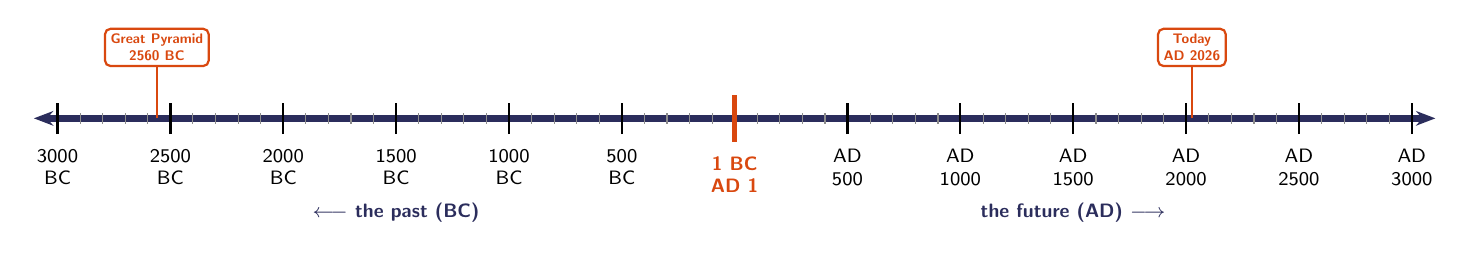
\begin{tikzpicture}
\draw[line width=2.4pt, ttdark, {Stealth[length=7pt]}-{Stealth[length=7pt]}] (-0.3,0) -- (17.50,0);
\draw[black!45] (0.000,-0.07) -- (0.000,0.07);
\draw[black!45] (0.287,-0.07) -- (0.287,0.07);
\draw[black!45] (0.573,-0.07) -- (0.573,0.07);
\draw[black!45] (0.860,-0.07) -- (0.860,0.07);
\draw[black!45] (1.147,-0.07) -- (1.147,0.07);
\draw[black!45] (1.434,-0.07) -- (1.434,0.07);
\draw[black!45] (1.720,-0.07) -- (1.720,0.07);
\draw[black!45] (2.007,-0.07) -- (2.007,0.07);
\draw[black!45] (2.294,-0.07) -- (2.294,0.07);
\draw[black!45] (2.580,-0.07) -- (2.580,0.07);
\draw[black!45] (2.867,-0.07) -- (2.867,0.07);
\draw[black!45] (3.154,-0.07) -- (3.154,0.07);
\draw[black!45] (3.441,-0.07) -- (3.441,0.07);
\draw[black!45] (3.727,-0.07) -- (3.727,0.07);
\draw[black!45] (4.014,-0.07) -- (4.014,0.07);
\draw[black!45] (4.301,-0.07) -- (4.301,0.07);
\draw[black!45] (4.587,-0.07) -- (4.587,0.07);
\draw[black!45] (4.874,-0.07) -- (4.874,0.07);
\draw[black!45] (5.161,-0.07) -- (5.161,0.07);
\draw[black!45] (5.448,-0.07) -- (5.448,0.07);
\draw[black!45] (5.734,-0.07) -- (5.734,0.07);
\draw[black!45] (6.021,-0.07) -- (6.021,0.07);
\draw[black!45] (6.308,-0.07) -- (6.308,0.07);
\draw[black!45] (6.594,-0.07) -- (6.594,0.07);
\draw[black!45] (6.881,-0.07) -- (6.881,0.07);
\draw[black!45] (7.168,-0.07) -- (7.168,0.07);
\draw[black!45] (7.455,-0.07) -- (7.455,0.07);
\draw[black!45] (7.741,-0.07) -- (7.741,0.07);
\draw[black!45] (8.028,-0.07) -- (8.028,0.07);
\draw[black!45] (8.315,-0.07) -- (8.315,0.07);
\draw[black!45] (8.601,-0.07) -- (8.601,0.07);
\draw[black!45] (8.888,-0.07) -- (8.888,0.07);
\draw[black!45] (9.175,-0.07) -- (9.175,0.07);
\draw[black!45] (9.462,-0.07) -- (9.462,0.07);
\draw[black!45] (9.748,-0.07) -- (9.748,0.07);
\draw[black!45] (10.035,-0.07) -- (10.035,0.07);
\draw[black!45] (10.322,-0.07) -- (10.322,0.07);
\draw[black!45] (10.608,-0.07) -- (10.608,0.07);
\draw[black!45] (10.895,-0.07) -- (10.895,0.07);
\draw[black!45] (11.182,-0.07) -- (11.182,0.07);
\draw[black!45] (11.469,-0.07) -- (11.469,0.07);
\draw[black!45] (11.755,-0.07) -- (11.755,0.07);
\draw[black!45] (12.042,-0.07) -- (12.042,0.07);
\draw[black!45] (12.329,-0.07) -- (12.329,0.07);
\draw[black!45] (12.615,-0.07) -- (12.615,0.07);
\draw[black!45] (12.902,-0.07) -- (12.902,0.07);
\draw[black!45] (13.189,-0.07) -- (13.189,0.07);
\draw[black!45] (13.476,-0.07) -- (13.476,0.07);
\draw[black!45] (13.762,-0.07) -- (13.762,0.07);
\draw[black!45] (14.049,-0.07) -- (14.049,0.07);
\draw[black!45] (14.336,-0.07) -- (14.336,0.07);
\draw[black!45] (14.622,-0.07) -- (14.622,0.07);
\draw[black!45] (14.909,-0.07) -- (14.909,0.07);
\draw[black!45] (15.196,-0.07) -- (15.196,0.07);
\draw[black!45] (15.483,-0.07) -- (15.483,0.07);
\draw[black!45] (15.769,-0.07) -- (15.769,0.07);
\draw[black!45] (16.056,-0.07) -- (16.056,0.07);
\draw[black!45] (16.343,-0.07) -- (16.343,0.07);
\draw[black!45] (16.629,-0.07) -- (16.629,0.07);
\draw[black!45] (16.916,-0.07) -- (16.916,0.07);
\draw[thick] (0.000,-0.2) -- (0.000,0.2);
\node[font=\scriptsize, below=2pt, align=center] at (0.000,-0.2) {3000\\BC};
\draw[thick] (1.434,-0.2) -- (1.434,0.2);
\node[font=\scriptsize, below=2pt, align=center] at (1.434,-0.2) {2500\\BC};
\draw[thick] (2.867,-0.2) -- (2.867,0.2);
\node[font=\scriptsize, below=2pt, align=center] at (2.867,-0.2) {2000\\BC};
\draw[thick] (4.301,-0.2) -- (4.301,0.2);
\node[font=\scriptsize, below=2pt, align=center] at (4.301,-0.2) {1500\\BC};
\draw[thick] (5.734,-0.2) -- (5.734,0.2);
\node[font=\scriptsize, below=2pt, align=center] at (5.734,-0.2) {1000\\BC};
\draw[thick] (7.168,-0.2) -- (7.168,0.2);
\node[font=\scriptsize, below=2pt, align=center] at (7.168,-0.2) {500\\BC};
\draw[ultra thick, ttaccent] (8.600,-0.3) -- (8.600,0.3);
\node[font=\scriptsize\bfseries, below=2pt, align=center, text=ttaccent] at (8.600,-0.3) {1 BC\\AD 1};
\draw[thick] (10.032,-0.2) -- (10.032,0.2);
\node[font=\scriptsize, below=2pt, align=center] at (10.032,-0.2) {AD\\500};
\draw[thick] (11.466,-0.2) -- (11.466,0.2);
\node[font=\scriptsize, below=2pt, align=center] at (11.466,-0.2) {AD\\1000};
\draw[thick] (12.899,-0.2) -- (12.899,0.2);
\node[font=\scriptsize, below=2pt, align=center] at (12.899,-0.2) {AD\\1500};
\draw[thick] (14.333,-0.2) -- (14.333,0.2);
\node[font=\scriptsize, below=2pt, align=center] at (14.333,-0.2) {AD\\2000};
\draw[thick] (15.766,-0.2) -- (15.766,0.2);
\node[font=\scriptsize, below=2pt, align=center] at (15.766,-0.2) {AD\\2500};
\draw[thick] (17.200,-0.2) -- (17.200,0.2);
\node[font=\scriptsize, below=2pt, align=center] at (17.200,-0.2) {AD\\3000};
\node[font=\scriptsize\bfseries, text=ttdark] at (4.298,-1.2) {$\longleftarrow$ the past (BC)};
\node[font=\scriptsize\bfseries, text=ttdark] at (12.899,-1.2) {the future (AD) $\longrightarrow$};
\draw[ttaccent, thick] (1.262,0) -- (1.262,0.7);
\node[flag, above] at (1.262,0.65) {Great Pyramid\\2560 BC};
\draw[ttaccent, thick] (14.407,0) -- (14.407,0.7);
\node[flag, above] at (14.407,0.65) {Today\\AD 2026};
\end{tikzpicture}\end{center}\vspace{6pt}

\ealpara{\ealkeytr{Garis waktu} yang diperbesar: 1000 \ealkeytr{Masehi} sampai 2100 \ealkeytr{Masehi}. Tanda kecil setiap 10 tahun (satu \ealkeytr{dekade}). Tanda besar setiap 100 tahun (satu \ealkeytr{abad}).}{}
{\small\bfseries The zoomed \ealkey{timeline}: \ealkey{AD} 1000 to \ealkey{AD} 2100}\par\vspace{18pt}

\begin{center}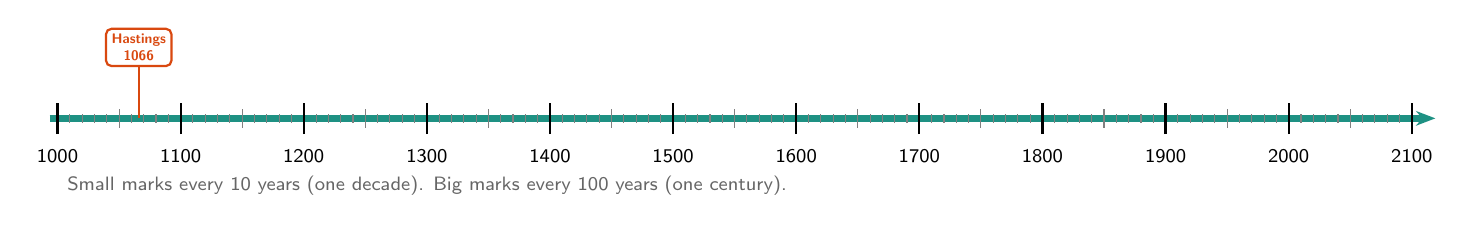
\begin{tikzpicture}
\draw[line width=2.4pt, ttglow!80!black, -{Stealth[length=7pt]}] (-0.1,0) -- (17.50,0);
\draw[thick] (0.000,-0.20) -- (0.000,0.20);
\node[font=\scriptsize, below=2pt] at (0.000,-0.2) {1000};
\draw[black!50] (0.156,-0.06) -- (0.156,0.06);
\draw[black!50] (0.313,-0.06) -- (0.313,0.06);
\draw[black!50] (0.469,-0.06) -- (0.469,0.06);
\draw[black!50] (0.625,-0.06) -- (0.625,0.06);
\draw[black!50] (0.782,-0.12) -- (0.782,0.12);
\draw[black!50] (0.938,-0.06) -- (0.938,0.06);
\draw[black!50] (1.095,-0.06) -- (1.095,0.06);
\draw[black!50] (1.251,-0.06) -- (1.251,0.06);
\draw[black!50] (1.407,-0.06) -- (1.407,0.06);
\draw[thick] (1.564,-0.20) -- (1.564,0.20);
\node[font=\scriptsize, below=2pt] at (1.564,-0.2) {1100};
\draw[black!50] (1.720,-0.06) -- (1.720,0.06);
\draw[black!50] (1.876,-0.06) -- (1.876,0.06);
\draw[black!50] (2.033,-0.06) -- (2.033,0.06);
\draw[black!50] (2.189,-0.06) -- (2.189,0.06);
\draw[black!50] (2.345,-0.12) -- (2.345,0.12);
\draw[black!50] (2.502,-0.06) -- (2.502,0.06);
\draw[black!50] (2.658,-0.06) -- (2.658,0.06);
\draw[black!50] (2.815,-0.06) -- (2.815,0.06);
\draw[black!50] (2.971,-0.06) -- (2.971,0.06);
\draw[thick] (3.127,-0.20) -- (3.127,0.20);
\node[font=\scriptsize, below=2pt] at (3.127,-0.2) {1200};
\draw[black!50] (3.284,-0.06) -- (3.284,0.06);
\draw[black!50] (3.440,-0.06) -- (3.440,0.06);
\draw[black!50] (3.596,-0.06) -- (3.596,0.06);
\draw[black!50] (3.753,-0.06) -- (3.753,0.06);
\draw[black!50] (3.909,-0.12) -- (3.909,0.12);
\draw[black!50] (4.065,-0.06) -- (4.065,0.06);
\draw[black!50] (4.222,-0.06) -- (4.222,0.06);
\draw[black!50] (4.378,-0.06) -- (4.378,0.06);
\draw[black!50] (4.535,-0.06) -- (4.535,0.06);
\draw[thick] (4.691,-0.20) -- (4.691,0.20);
\node[font=\scriptsize, below=2pt] at (4.691,-0.2) {1300};
\draw[black!50] (4.847,-0.06) -- (4.847,0.06);
\draw[black!50] (5.004,-0.06) -- (5.004,0.06);
\draw[black!50] (5.160,-0.06) -- (5.160,0.06);
\draw[black!50] (5.316,-0.06) -- (5.316,0.06);
\draw[black!50] (5.473,-0.12) -- (5.473,0.12);
\draw[black!50] (5.629,-0.06) -- (5.629,0.06);
\draw[black!50] (5.785,-0.06) -- (5.785,0.06);
\draw[black!50] (5.942,-0.06) -- (5.942,0.06);
\draw[black!50] (6.098,-0.06) -- (6.098,0.06);
\draw[thick] (6.255,-0.20) -- (6.255,0.20);
\node[font=\scriptsize, below=2pt] at (6.255,-0.2) {1400};
\draw[black!50] (6.411,-0.06) -- (6.411,0.06);
\draw[black!50] (6.567,-0.06) -- (6.567,0.06);
\draw[black!50] (6.724,-0.06) -- (6.724,0.06);
\draw[black!50] (6.880,-0.06) -- (6.880,0.06);
\draw[black!50] (7.036,-0.12) -- (7.036,0.12);
\draw[black!50] (7.193,-0.06) -- (7.193,0.06);
\draw[black!50] (7.349,-0.06) -- (7.349,0.06);
\draw[black!50] (7.505,-0.06) -- (7.505,0.06);
\draw[black!50] (7.662,-0.06) -- (7.662,0.06);
\draw[thick] (7.818,-0.20) -- (7.818,0.20);
\node[font=\scriptsize, below=2pt] at (7.818,-0.2) {1500};
\draw[black!50] (7.975,-0.06) -- (7.975,0.06);
\draw[black!50] (8.131,-0.06) -- (8.131,0.06);
\draw[black!50] (8.287,-0.06) -- (8.287,0.06);
\draw[black!50] (8.444,-0.06) -- (8.444,0.06);
\draw[black!50] (8.600,-0.12) -- (8.600,0.12);
\draw[black!50] (8.756,-0.06) -- (8.756,0.06);
\draw[black!50] (8.913,-0.06) -- (8.913,0.06);
\draw[black!50] (9.069,-0.06) -- (9.069,0.06);
\draw[black!50] (9.225,-0.06) -- (9.225,0.06);
\draw[thick] (9.382,-0.20) -- (9.382,0.20);
\node[font=\scriptsize, below=2pt] at (9.382,-0.2) {1600};
\draw[black!50] (9.538,-0.06) -- (9.538,0.06);
\draw[black!50] (9.695,-0.06) -- (9.695,0.06);
\draw[black!50] (9.851,-0.06) -- (9.851,0.06);
\draw[black!50] (10.007,-0.06) -- (10.007,0.06);
\draw[black!50] (10.164,-0.12) -- (10.164,0.12);
\draw[black!50] (10.320,-0.06) -- (10.320,0.06);
\draw[black!50] (10.476,-0.06) -- (10.476,0.06);
\draw[black!50] (10.633,-0.06) -- (10.633,0.06);
\draw[black!50] (10.789,-0.06) -- (10.789,0.06);
\draw[thick] (10.945,-0.20) -- (10.945,0.20);
\node[font=\scriptsize, below=2pt] at (10.945,-0.2) {1700};
\draw[black!50] (11.102,-0.06) -- (11.102,0.06);
\draw[black!50] (11.258,-0.06) -- (11.258,0.06);
\draw[black!50] (11.415,-0.06) -- (11.415,0.06);
\draw[black!50] (11.571,-0.06) -- (11.571,0.06);
\draw[black!50] (11.727,-0.12) -- (11.727,0.12);
\draw[black!50] (11.884,-0.06) -- (11.884,0.06);
\draw[black!50] (12.040,-0.06) -- (12.040,0.06);
\draw[black!50] (12.196,-0.06) -- (12.196,0.06);
\draw[black!50] (12.353,-0.06) -- (12.353,0.06);
\draw[thick] (12.509,-0.20) -- (12.509,0.20);
\node[font=\scriptsize, below=2pt] at (12.509,-0.2) {1800};
\draw[black!50] (12.665,-0.06) -- (12.665,0.06);
\draw[black!50] (12.822,-0.06) -- (12.822,0.06);
\draw[black!50] (12.978,-0.06) -- (12.978,0.06);
\draw[black!50] (13.135,-0.06) -- (13.135,0.06);
\draw[black!50] (13.291,-0.12) -- (13.291,0.12);
\draw[black!50] (13.447,-0.06) -- (13.447,0.06);
\draw[black!50] (13.604,-0.06) -- (13.604,0.06);
\draw[black!50] (13.760,-0.06) -- (13.760,0.06);
\draw[black!50] (13.916,-0.06) -- (13.916,0.06);
\draw[thick] (14.073,-0.20) -- (14.073,0.20);
\node[font=\scriptsize, below=2pt] at (14.073,-0.2) {1900};
\draw[black!50] (14.229,-0.06) -- (14.229,0.06);
\draw[black!50] (14.385,-0.06) -- (14.385,0.06);
\draw[black!50] (14.542,-0.06) -- (14.542,0.06);
\draw[black!50] (14.698,-0.06) -- (14.698,0.06);
\draw[black!50] (14.855,-0.12) -- (14.855,0.12);
\draw[black!50] (15.011,-0.06) -- (15.011,0.06);
\draw[black!50] (15.167,-0.06) -- (15.167,0.06);
\draw[black!50] (15.324,-0.06) -- (15.324,0.06);
\draw[black!50] (15.480,-0.06) -- (15.480,0.06);
\draw[thick] (15.636,-0.20) -- (15.636,0.20);
\node[font=\scriptsize, below=2pt] at (15.636,-0.2) {2000};
\draw[black!50] (15.793,-0.06) -- (15.793,0.06);
\draw[black!50] (15.949,-0.06) -- (15.949,0.06);
\draw[black!50] (16.105,-0.06) -- (16.105,0.06);
\draw[black!50] (16.262,-0.06) -- (16.262,0.06);
\draw[black!50] (16.418,-0.12) -- (16.418,0.12);
\draw[black!50] (16.575,-0.06) -- (16.575,0.06);
\draw[black!50] (16.731,-0.06) -- (16.731,0.06);
\draw[black!50] (16.887,-0.06) -- (16.887,0.06);
\draw[black!50] (17.044,-0.06) -- (17.044,0.06);
\draw[thick] (17.200,-0.20) -- (17.200,0.20);
\node[font=\scriptsize, below=2pt] at (17.200,-0.2) {2100};
\node[font=\scriptsize, text=black!60, anchor=west] at (0,-0.85) {Small marks every 10 years (one decade). Big marks every 100 years (one century).};
\draw[ttaccent, thick] (1.032,0) -- (1.032,0.7);
\node[flag, above] at (1.032,0.65) {Hastings\\1066};
\end{tikzpicture}\end{center}

{\small \begin{enumerate}[label=\textbf{\arabic*.}, leftmargin=*, itemsep=5pt, topsep=4pt, start=1]
\item \ealpara{Tandai ini pada \ealkeytr{garis waktu} besar dengan tanda silang dan label: \quad Tutankhamun meninggal \textbf{1323 \ealkeytr{Sebelum Masehi}} \quad Olimpiade Pertama \textbf{776 \ealkeytr{Sebelum Masehi}} \quad Romawi menyerbu Inggris \textbf{43 \ealkeytr{Masehi}} \quad Pertempuran Hastings \textbf{1066 \ealkeytr{Masehi}}}{Mark these on the big \ealkey{timeline} with a cross and a label: \quad Tutankhamun dies \textbf{1323 \ealkey{BC}} \quad First Olympic Games \textbf{776 \ealkey{BC}} \quad Romans invade Britain \textbf{\ealkey{AD} 43} \quad Battle of Hastings \textbf{\ealkey{AD} 1066}}
\item \ealpara{Berapa tahun yang lalu (dari 2026) \ldots}{How many years ago (from 2026) was \ldots}
\ealpara{(a) Pertempuran Hastings? \aline \quad (b) Invasi Romawi? \aline\\[5pt](c) Olimpiade pertama? \aline \quad (d) Piramida Agung? \aline}{}
\begin{tabular}{@{}l@{\ }l@{\qquad}l@{\ }l}(a) the Battle of Hastings? & \aline & (b) the Roman invasion? & \aline\\[5pt](c) the first Olympic Games? & \aline & (d) the Great Pyramid? & \aline\end{tabular}
\item \ealpara{Tulis jawabanmu untuk 2(a) dalam \ealkeytr{abad} dan \ealkeytr{dekade}: \lline}{Write your answer to 2(a) in \ealkey{centuries} and \ealkey{decades}: \lline}
\item \ealpara{Di mana (kapan!) mesin mendarat? Tandai ini pada \ealkeytr{garis waktu} besar juga.}{Where (when!) does the machine land? Mark these on the big \ealkey{timeline} too.}
\ealpara{dari 2026: \dial{BACK}{3}{MILLENNIA} mendarat di \lline; dari 2026: \dial{FORWARD}{5}{CENTURIES} mendarat di \lline; dari 2026: \dial{BACK}{25}{CENTURIES} mendarat di \lline}{}
\begin{tabular}{@{}l@{\ }l}from 2026: \dial{BACK}{3}{MILLENNIA} & lands in \lline\\[5pt]from 2026: \dial{FORWARD}{5}{CENTURIES} & lands in \lline\\[5pt]from 2026: \dial{BACK}{25}{CENTURIES} & lands in \lline\end{tabular}
\item \ealpara{\textbf{Perbesar:} tandai ini pada \ealkeytr{garis waktu} yang diperbesar: \quad Magna Carta \textbf{1215} \quad Kebakaran Besar London \textbf{1666} \quad Pendaratan Bulan \textbf{1969} \quad Hari ini \textbf{2026}}{\textbf{Zoom in:} mark these on the zoomed \ealkey{timeline}: \quad Magna Carta \textbf{1215} \quad Great Fire of London \textbf{1666} \quad Moon landing \textbf{1969} \quad Today \textbf{2026}}
\item \ealpara{Berapa tahun dari (a) Magna Carta ke Kebakaran Besar? \aline\quad (b) Pendaratan Bulan sampai hari ini? \aline}{How many years from (a) Magna Carta to the Great Fire? \aline\quad (b) the Moon landing to today? \aline}
\item \ealpara{Apakah Kebakaran Besar London lebih dekat waktunya ke Pertempuran Hastings, atau ke hari ini? Tunjukkan bagaimana kamu tahu.}{Is the Great Fire of London closer in time to the Battle of Hastings, or to today? Show how you know.}\par\vspace{4pt}\rule{\linewidth}{0.4pt}
\end{enumerate}}

\clearpage

\ealpara{Bagian D \quad Catatan misi --- pulang ke rumah}{}
\banner{Part D \quad Mission log --- getting home}\par\smallskip

\ealpara{Dr Chrono berangkat dari \textbf{2026 \ealkeytr{Masehi}} dan melakukan empat lompatan. Baterainya mulai dari \textbf{100\%}, dan setiap \ealkeytr{abad} perjalanan (maju atau mundur) menggunakan \textbf{2\%} dari baterai.}{Dr Chrono sets off from \textbf{\ealkey{AD} 2026} and makes four jumps. Her battery starts at \textbf{100\%}, and every \textbf{\ealkey{century}} of travel (forwards or backwards) uses \textbf{2\%} of the battery.}\par\medskip

\ealpara{Tabel: \textbf{Lompatan}, \textbf{Dial}, \textbf{Dari}, \textbf{Mendarat di}}{}
\begin{center}{\small\begin{tabular}{c|c|p{3.2cm}|p{3.2cm}}\textbf{Jump} & \textbf{Dial} & \textbf{From} & \textbf{Lands in}\\\hline
1 & \dial{BACK}{3}{CENTURIES} & AD 2026 & \\[3pt]\hline
2 & \dial{FORWARD}{25}{YEARS} &  & \\[3pt]\hline
3 & \dial{BACK}{2}{MILLENNIA} &  & \\[3pt]\hline
4 & \dial{FORWARD}{1500}{YEARS} &  & \\[3pt]\hline\end{tabular}}\end{center}

{\small \begin{enumerate}[label=\textbf{\arabic*.}, leftmargin=*, itemsep=5pt, topsep=4pt, start=1]
\item \ealpara{Lompatan tunggal apa yang akan membawa Dr Chrono langsung pulang ke 2026 \ealkeytr{Masehi}? \quad MAJU atau MUNDUR? \aline\quad Berapa tahun? \aline}{What single jump would take Dr Chrono straight home to \ealkey{AD} 2026? \quad FORWARD or BACK? \aline\quad How many years? \aline}
\item \ealpara{Berapa tahun total yang dia tempuh dalam lompatan 1--4? \aline\quad Berapa \ealkeytr{abad} itu? \aline}{How many years did she travel in jumps 1--4 altogether? \aline\quad How many \ealkey{centuries} is that? \aline}
\item \ealpara{Berapa banyak baterai yang telah dia gunakan sejauh ini? \aline\quad Berapa yang tersisa? \aline}{How much battery has she used so far? \aline\quad How much is left? \aline}
\item \ealpara{Apakah baterainya cukup untuk melakukan lompatan pulang? Tunjukkan perhitunganmu.}{Does she have enough battery to make the jump home? Show your working.}\par\vspace{4pt}\rule{\linewidth}{0.4pt}
\item \ealpara{\textbf{Rancang sebuah misi:} rencanakan tiga lompatan yang mengunjungi Piramida Agung, Pertempuran Hastings, dan Pendaratan Bulan, lalu pulang. Tulis pengaturan dialmu dan hitung baterai yang digunakan.}{\textbf{Design a mission:} plan three jumps that visit the Great Pyramid, the Battle of Hastings and the Moon landing, then come home. Write your dial settings and work out the battery used.}\par\medskip
\ealpara{Tabel: \textbf{Lompatan}, \textbf{Pengaturan dial}, \textbf{Mendarat di}, \textbf{Baterai yang digunakan}; \textbf{Total baterai yang digunakan}}{}
\begin{center}\begin{tabular}{c|p{3.4cm}|p{3.4cm}|p{3.4cm}}\textbf{Jump} & \textbf{Dial setting} & \textbf{Lands in} & \textbf{Battery used}\\\hline1 & & & \\[10pt]\hline 2 & & & \\[10pt]\hline 3 & & & \\[10pt]\hline Home & & & \\[10pt]\hline\multicolumn{3}{r|}{\textbf{Total battery used}} & \\[10pt]\hline\end{tabular}\end{center}
\end{enumerate}}

\clearpage\enlargethispage{3\baselineskip}

\ealpara{Jawaban}{}
\begin{center}{\LARGE\bfseries Answers}\end{center}\vspace{-6pt}

\ealpara{Bagian A \quad Lompatan \ealkeytr{kalender} --- lompatan kecil}{}
\banner{Part A \quad \ealkey{Calendar} hops --- small jumps}\par\smallskip

{\small \begin{enumerate}[label=\textbf{\arabic*.}, leftmargin=*, itemsep=5pt, topsep=4pt, start=1]
\item \ealpara{\dial{FORWARD}{1}{WEEK} \quad Hari dan tanggal: \lline}{\dial{FORWARD}{1}{WEEK} \quad Day and date: \lline}
\ealpara{Sabtu, 7 November 2026}{\ans{Saturday 7 November 2026}}
\item \ealpara{\dial{FORWARD}{10}{DAYS} \quad Hari dan tanggal: \lline}{\dial{FORWARD}{10}{DAYS} \quad Day and date: \lline}
\ealpara{Selasa, 10 November 2026}{\ans{Tuesday 10 November 2026}}
\item \ealpara{\dial{BACK}{2}{WEEKS} \quad Hari dan tanggal: \lline}{\dial{BACK}{2}{WEEKS} \quad Day and date: \lline}
\ealpara{Sabtu, 17 Oktober 2026}{\ans{Saturday 17 October 2026}}
\item \ealpara{\dial{FORWARD}{3 WEEKS}{+ 2 DAYS} \quad Hari dan tanggal: \lline}{\dial{FORWARD}{3 WEEKS}{+ 2 DAYS} \quad Day and date: \lline}
\ealpara{Senin, 23 November 2026}{\ans{Monday 23 November 2026}}
\item \ealpara{\dial{BACK}{45}{DAYS} \quad Hari dan tanggal: \lline}{\dial{BACK}{45}{DAYS} \quad Day and date: \lline}
\ealpara{Rabu, 16 September 2026}{\ans{Wednesday 16 September 2026}}
\item \ealpara{\dial{FORWARD}{100}{HOURS} \quad Hari, tanggal \emph{dan waktu}: \lline}{\dial{FORWARD}{100}{HOURS} \quad Day, date \emph{and time}: \lline}
\ealpara{Rabu, 4 November 2026 pukul 14.00 (100 jam = 4 hari 4 jam)}{\ans{Wednesday 4 November 2026 at 14:00 (100 hours = 4 days 4 hours)}}
\item \ealpara{Dr Chrono ingin menonton kembang api pada Malam Bonfire (5 November) lalu melompat ke Hari Natal (25 Desember). Berapa hari ke depan itu? \aline\ \ Tulis dalam minggu dan hari: \aline}{Dr Chrono wants to watch the fireworks on Bonfire Night (5 November) and then jump to Christmas Day (25 December). How many days forward is that? \aline\ \ Write it in weeks and days: \aline}
\ealpara{50 hari = 7 minggu 1 hari}{\ans{50 days = 7 weeks 1 day}}
\item \ealpara{Dial macet sehingga hanya bisa melompat dalam \textbf{minggu utuh}. Mulai dari hari ini, dapatkah Dr Chrono mendarat tepat pada Hari Natal? Jelaskan, dan sebutkan dua tanggal terdekat Natal yang \emph{dapat} dicapai.}{The dial gets stuck so it can only jump in \textbf{whole weeks}. Starting from today, can Dr Chrono land exactly on Christmas Day? Explain, and say which two dates nearest Christmas it \emph{can} reach.}\par\vspace{4pt}\rule{\linewidth}{0.4pt}
\ealpara{Tidak. 31 Okt sampai 25 Des adalah 55 hari, bukan \ealkeytr{kelipatan} 7. Minggu utuh dari hari Sabtu selalu mendarat pada hari Sabtu: Sabtu 19 Des (7 minggu) atau Sabtu 26 Des (8 minggu).}{\ans{No. 31 Oct to 25 Dec is 55 days, not a \ealkey{multiple} of 7. Whole weeks from a Saturday always land on a Saturday: Sat 19 Dec (7 weeks) or Sat 26 Dec (8 weeks).}}
\item \ealpara{\textbf{Pendaratan seram:} Mesin Dr Chrono selalu rusak pada hari Jumat tanggal 13. Tanggal mana pada \ealkeytr{kalender} ini yang harus dia hindari? \lline}{\textbf{Spooky landing:} Dr Chrono's machine always breaks down on a Friday the 13th. Which date on these \ealkey{calendars} should she avoid? \lline}
\ealpara{Jumat, 13 November 2026}{\ans{Friday 13 November 2026}}
\end{enumerate}}

\ealpara{Bagian B \quad Stasiun \ealkeytr{konversi} --- lompatan sedang}{}
\banner{Part B \quad \ealkey{Conversion} station --- medium jumps}\par\smallskip

\ealpara{\textbf{1.} Ubah: 3 minggu = 21 hari; 4 \ealkeytr{abad} = 40 \ealkeytr{dekade}; 2 hari = 48 jam; 2 \ealkeytr{milenium} = 20 \ealkeytr{abad}; 180 menit = 3 jam; 7200 detik = 2 jam; 5 \ealkeytr{dekade} = 50 tahun; 3 hari = 4320 menit}{}
{\small\begin{tabular}{rclp{1.6cm}p{0.6cm}rcll}3 weeks & = & \ans{21} & days && 4 \ealkey{centuries} & = & \ans{40} & \ealkey{decades}\\[4pt]
2 days & = & \ans{48} & hours && 2 \ealkey{millennia} & = & \ans{20} & \ealkey{centuries}\\[4pt]
180 minutes & = & \ans{3} & hours && 7200 seconds & = & \ans{2} & hours\\[4pt]
5 \ealkey{decades} & = & \ans{50} & years && 3 days & = & \ans{4320} & minutes\\[4pt]\end{tabular}}\par\medskip

{\small \begin{enumerate}[label=\textbf{\arabic*.}, leftmargin=*, itemsep=5pt, topsep=4pt, start=2]
\item \ealpara{Tulis setiap bacaan dial dengan cara yang lebih masuk akal.}{Write each dial reading in a more sensible way.}
\ealpara{\dial{FORWARD}{72}{HOURS} = \rule{3.5cm}{0.4pt} hari; \dial{FORWARD}{420}{DAYS} = \rule{3.5cm}{0.4pt} minggu; \dial{BACK}{1000}{HOURS} = \rule{1.5cm}{0.4pt} hari dan \rule{1.5cm}{0.4pt} jam; \dial{BACK}{1000000}{SECONDS} \textbf{Tantangan:} = \rule{0.8cm}{0.4pt} h \rule{0.8cm}{0.4pt} j \rule{0.8cm}{0.4pt} mnt \rule{0.8cm}{0.4pt} dtk}{}
\begin{tabular}{@{}ll}\dial{FORWARD}{72}{HOURS} & = \rule{3.5cm}{0.4pt} days\\[5pt]\dial{FORWARD}{420}{DAYS} & = \rule{3.5cm}{0.4pt} weeks\\[5pt]\dial{BACK}{1000}{HOURS} & = \rule{1.5cm}{0.4pt} days and \rule{1.5cm}{0.4pt} hours\\[5pt]\dial{BACK}{1000000}{SECONDS} & \textbf{Challenge:} = \rule{0.8cm}{0.4pt} d \rule{0.8cm}{0.4pt} h \rule{0.8cm}{0.4pt} min \rule{0.8cm}{0.4pt} s\end{tabular}
\ealpara{3 hari;\quad 60 minggu;\quad 41 hari 16 jam;\quad 11 h 13 j 46 mnt 40 dtk}{\ans{3 days;\quad 60 weeks;\quad 41 days 16 hours;\quad 11 d 13 h 46 min 40 s}}
\item \ealpara{Dr Chrono mendarat pada \textbf{29 Februari}. Tahun mana saja berikut yang mungkin? Lingkari: \quad 2028 \quad 2030 \quad 2100 \quad 2400}{Dr Chrono lands on \textbf{29 February}. Which of these years could it be? Circle them: \quad 2028 \quad 2030 \quad 2100 \quad 2400}
\ealpara{2028 dan 2400 (2030 tidak \ealkeytr{habis dibagi} 4; 2100 adalah \ealkeytr{tahun abad} yang tidak \ealkeytr{habis dibagi} 400)}{\ans{2028 and 2400 (2030 is not \ealkey{divisible} by 4; 2100 is a \ealkey{century year} not \ealkey{divisible} by 400)}}
\item \ealpara{Urutkan lompatan-lompatan ini dari \textbf{terpendek} ke \textbf{terpanjang}: \dial{JUMP}{1000}{HOURS}\ \ \dial{JUMP}{6}{WEEKS}\ \ \dial{JUMP}{50000}{MINUTES}\quad \dial{JUMP}{1000000}{SECONDS}\ \ \dial{JUMP}{0.1}{YEARS}}{Put these jumps in order from \textbf{shortest} to \textbf{longest}: \dial{JUMP}{1000}{HOURS}\ \ \dial{JUMP}{6}{WEEKS}\ \ \dial{JUMP}{50000}{MINUTES}\quad \dial{JUMP}{1000000}{SECONDS}\ \ \dial{JUMP}{0.1}{YEARS}}\par\vspace{6pt}\rule{\linewidth}{0.4pt}
\ealpara{1\,000\,000 dtk ($\approx$ 11,6 hari) $<$ 50\,000 mnt ($\approx$ 34,7 hari) $<$ 0,1 tahun (36,5 hari) $<$ 1000 jam ($\approx$ 41,7 hari) $<$ 6 minggu (42 hari)}{\ans{1\,000\,000 s ($\approx$ 11.6 days) $<$ 50\,000 min ($\approx$ 34.7 days) $<$ 0.1 years (36.5 days) $<$ 1000 hours ($\approx$ 41.7 days) $<$ 6 weeks (42 days)}}
\end{enumerate}}

\clearpage

\ealpara{Bagian C \quad Lompatan \ealkeytr{garis waktu} --- lompatan raksasa}{}
\banner{Part C \quad \ealkey{Timeline} jumps --- giant leaps}\par\smallskip

\ealpara{\ealkeytr{Garis waktu} besar: 3000 \ealkeytr{Sebelum Masehi} sampai 3000 \ealkeytr{Masehi}. Tanda kecil setiap \ealkeytr{abad}.}{}
{\small\bfseries The \ealkey{timeline}: 3000 \ealkey{BC} to \ealkey{AD} 3000} \hfill {\scriptsize small marks every \ealkey{century}}\par\vspace{18pt}

\begin{center}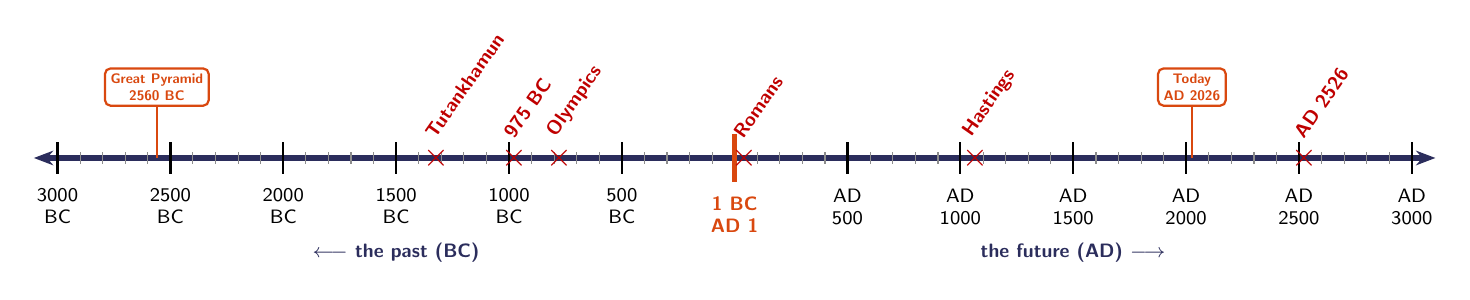
\begin{tikzpicture}
\draw[line width=2.4pt, ttdark, {Stealth[length=7pt]}-{Stealth[length=7pt]}] (-0.3,0) -- (17.50,0);
\draw[black!45] (0.000,-0.07) -- (0.000,0.07);
\draw[black!45] (0.287,-0.07) -- (0.287,0.07);
\draw[black!45] (0.573,-0.07) -- (0.573,0.07);
\draw[black!45] (0.860,-0.07) -- (0.860,0.07);
\draw[black!45] (1.147,-0.07) -- (1.147,0.07);
\draw[black!45] (1.434,-0.07) -- (1.434,0.07);
\draw[black!45] (1.720,-0.07) -- (1.720,0.07);
\draw[black!45] (2.007,-0.07) -- (2.007,0.07);
\draw[black!45] (2.294,-0.07) -- (2.294,0.07);
\draw[black!45] (2.580,-0.07) -- (2.580,0.07);
\draw[black!45] (2.867,-0.07) -- (2.867,0.07);
\draw[black!45] (3.154,-0.07) -- (3.154,0.07);
\draw[black!45] (3.441,-0.07) -- (3.441,0.07);
\draw[black!45] (3.727,-0.07) -- (3.727,0.07);
\draw[black!45] (4.014,-0.07) -- (4.014,0.07);
\draw[black!45] (4.301,-0.07) -- (4.301,0.07);
\draw[black!45] (4.587,-0.07) -- (4.587,0.07);
\draw[black!45] (4.874,-0.07) -- (4.874,0.07);
\draw[black!45] (5.161,-0.07) -- (5.161,0.07);
\draw[black!45] (5.448,-0.07) -- (5.448,0.07);
\draw[black!45] (5.734,-0.07) -- (5.734,0.07);
\draw[black!45] (6.021,-0.07) -- (6.021,0.07);
\draw[black!45] (6.308,-0.07) -- (6.308,0.07);
\draw[black!45] (6.594,-0.07) -- (6.594,0.07);
\draw[black!45] (6.881,-0.07) -- (6.881,0.07);
\draw[black!45] (7.168,-0.07) -- (7.168,0.07);
\draw[black!45] (7.455,-0.07) -- (7.455,0.07);
\draw[black!45] (7.741,-0.07) -- (7.741,0.07);
\draw[black!45] (8.028,-0.07) -- (8.028,0.07);
\draw[black!45] (8.315,-0.07) -- (8.315,0.07);
\draw[black!45] (8.601,-0.07) -- (8.601,0.07);
\draw[black!45] (8.888,-0.07) -- (8.888,0.07);
\draw[black!45] (9.175,-0.07) -- (9.175,0.07);
\draw[black!45] (9.462,-0.07) -- (9.462,0.07);
\draw[black!45] (9.748,-0.07) -- (9.748,0.07);
\draw[black!45] (10.035,-0.07) -- (10.035,0.07);
\draw[black!45] (10.322,-0.07) -- (10.322,0.07);
\draw[black!45] (10.608,-0.07) -- (10.608,0.07);
\draw[black!45] (10.895,-0.07) -- (10.895,0.07);
\draw[black!45] (11.182,-0.07) -- (11.182,0.07);
\draw[black!45] (11.469,-0.07) -- (11.469,0.07);
\draw[black!45] (11.755,-0.07) -- (11.755,0.07);
\draw[black!45] (12.042,-0.07) -- (12.042,0.07);
\draw[black!45] (12.329,-0.07) -- (12.329,0.07);
\draw[black!45] (12.615,-0.07) -- (12.615,0.07);
\draw[black!45] (12.902,-0.07) -- (12.902,0.07);
\draw[black!45] (13.189,-0.07) -- (13.189,0.07);
\draw[black!45] (13.476,-0.07) -- (13.476,0.07);
\draw[black!45] (13.762,-0.07) -- (13.762,0.07);
\draw[black!45] (14.049,-0.07) -- (14.049,0.07);
\draw[black!45] (14.336,-0.07) -- (14.336,0.07);
\draw[black!45] (14.622,-0.07) -- (14.622,0.07);
\draw[black!45] (14.909,-0.07) -- (14.909,0.07);
\draw[black!45] (15.196,-0.07) -- (15.196,0.07);
\draw[black!45] (15.483,-0.07) -- (15.483,0.07);
\draw[black!45] (15.769,-0.07) -- (15.769,0.07);
\draw[black!45] (16.056,-0.07) -- (16.056,0.07);
\draw[black!45] (16.343,-0.07) -- (16.343,0.07);
\draw[black!45] (16.629,-0.07) -- (16.629,0.07);
\draw[black!45] (16.916,-0.07) -- (16.916,0.07);
\draw[thick] (0.000,-0.2) -- (0.000,0.2);
\node[font=\scriptsize, below=2pt, align=center] at (0.000,-0.2) {3000\\BC};
\draw[thick] (1.434,-0.2) -- (1.434,0.2);
\node[font=\scriptsize, below=2pt, align=center] at (1.434,-0.2) {2500\\BC};
\draw[thick] (2.867,-0.2) -- (2.867,0.2);
\node[font=\scriptsize, below=2pt, align=center] at (2.867,-0.2) {2000\\BC};
\draw[thick] (4.301,-0.2) -- (4.301,0.2);
\node[font=\scriptsize, below=2pt, align=center] at (4.301,-0.2) {1500\\BC};
\draw[thick] (5.734,-0.2) -- (5.734,0.2);
\node[font=\scriptsize, below=2pt, align=center] at (5.734,-0.2) {1000\\BC};
\draw[thick] (7.168,-0.2) -- (7.168,0.2);
\node[font=\scriptsize, below=2pt, align=center] at (7.168,-0.2) {500\\BC};
\draw[ultra thick, ttaccent] (8.600,-0.3) -- (8.600,0.3);
\node[font=\scriptsize\bfseries, below=2pt, align=center, text=ttaccent] at (8.600,-0.3) {1 BC\\AD 1};
\draw[thick] (10.032,-0.2) -- (10.032,0.2);
\node[font=\scriptsize, below=2pt, align=center] at (10.032,-0.2) {AD\\500};
\draw[thick] (11.466,-0.2) -- (11.466,0.2);
\node[font=\scriptsize, below=2pt, align=center] at (11.466,-0.2) {AD\\1000};
\draw[thick] (12.899,-0.2) -- (12.899,0.2);
\node[font=\scriptsize, below=2pt, align=center] at (12.899,-0.2) {AD\\1500};
\draw[thick] (14.333,-0.2) -- (14.333,0.2);
\node[font=\scriptsize, below=2pt, align=center] at (14.333,-0.2) {AD\\2000};
\draw[thick] (15.766,-0.2) -- (15.766,0.2);
\node[font=\scriptsize, below=2pt, align=center] at (15.766,-0.2) {AD\\2500};
\draw[thick] (17.200,-0.2) -- (17.200,0.2);
\node[font=\scriptsize, below=2pt, align=center] at (17.200,-0.2) {AD\\3000};
\node[font=\scriptsize\bfseries, text=ttdark] at (4.298,-1.2) {$\longleftarrow$ the past (BC)};
\node[font=\scriptsize\bfseries, text=ttdark] at (12.899,-1.2) {the future (AD) $\longrightarrow$};
\draw[ttaccent, thick] (1.262,0) -- (1.262,0.7);
\node[flag, above] at (1.262,0.65) {Great Pyramid\\2560 BC};
\draw[ttaccent, thick] (14.407,0) -- (14.407,0.7);
\node[flag, above] at (14.407,0.65) {Today\\AD 2026};
\node[text=red!75!black, font=\large\bfseries] at (4.808,0) {$\times$};
\node[text=red!75!black, font=\scriptsize\bfseries, rotate=55, anchor=south west, inner sep=1pt] at (4.808,0.18) {Tutankhamun};
\node[text=red!75!black, font=\large\bfseries] at (6.377,0) {$\times$};
\node[text=red!75!black, font=\scriptsize\bfseries, rotate=55, anchor=south west, inner sep=1pt] at (6.377,0.18) {Olympics};
\node[text=red!75!black, font=\large\bfseries] at (8.722,0) {$\times$};
\node[text=red!75!black, font=\scriptsize\bfseries, rotate=55, anchor=south west, inner sep=1pt] at (8.722,0.18) {Romans};
\node[text=red!75!black, font=\large\bfseries] at (11.655,0) {$\times$};
\node[text=red!75!black, font=\scriptsize\bfseries, rotate=55, anchor=south west, inner sep=1pt] at (11.655,0.18) {Hastings};
\node[text=red!75!black, font=\large\bfseries] at (5.806,0) {$\times$};
\node[text=red!75!black, font=\scriptsize\bfseries, rotate=55, anchor=south west, inner sep=1pt] at (5.806,0.18) {975 BC};
\node[text=red!75!black, font=\large\bfseries] at (15.841,0) {$\times$};
\node[text=red!75!black, font=\scriptsize\bfseries, rotate=55, anchor=south west, inner sep=1pt] at (15.841,0.18) {AD 2526};
\end{tikzpicture}\end{center}\vspace{6pt}

\ealpara{\ealkeytr{Garis waktu} yang diperbesar: 1000 \ealkeytr{Masehi} sampai 2100 \ealkeytr{Masehi}. Tanda kecil setiap 10 tahun (satu \ealkeytr{dekade}). Tanda besar setiap 100 tahun (satu \ealkeytr{abad}).}{}
{\small\bfseries The zoomed \ealkey{timeline}: \ealkey{AD} 1000 to \ealkey{AD} 2100}\par\vspace{18pt}

\begin{center}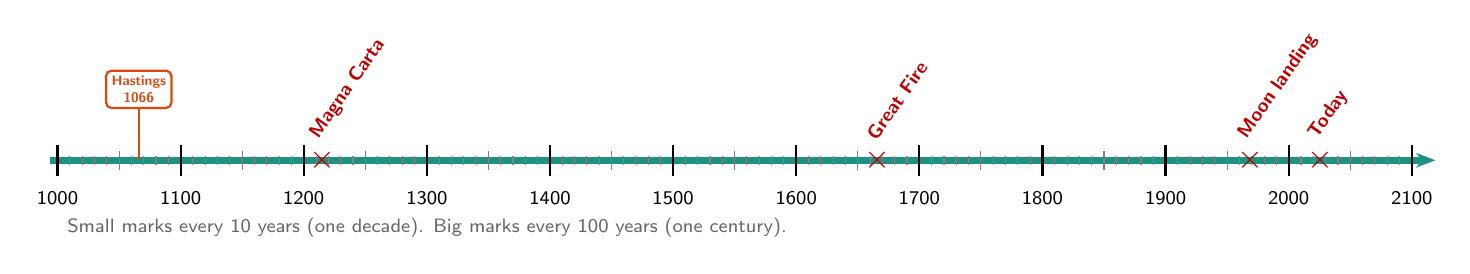
\begin{tikzpicture}
\draw[line width=2.4pt, ttglow!80!black, -{Stealth[length=7pt]}] (-0.1,0) -- (17.50,0);
\draw[thick] (0.000,-0.20) -- (0.000,0.20);
\node[font=\scriptsize, below=2pt] at (0.000,-0.2) {1000};
\draw[black!50] (0.156,-0.06) -- (0.156,0.06);
\draw[black!50] (0.313,-0.06) -- (0.313,0.06);
\draw[black!50] (0.469,-0.06) -- (0.469,0.06);
\draw[black!50] (0.625,-0.06) -- (0.625,0.06);
\draw[black!50] (0.782,-0.12) -- (0.782,0.12);
\draw[black!50] (0.938,-0.06) -- (0.938,0.06);
\draw[black!50] (1.095,-0.06) -- (1.095,0.06);
\draw[black!50] (1.251,-0.06) -- (1.251,0.06);
\draw[black!50] (1.407,-0.06) -- (1.407,0.06);
\draw[thick] (1.564,-0.20) -- (1.564,0.20);
\node[font=\scriptsize, below=2pt] at (1.564,-0.2) {1100};
\draw[black!50] (1.720,-0.06) -- (1.720,0.06);
\draw[black!50] (1.876,-0.06) -- (1.876,0.06);
\draw[black!50] (2.033,-0.06) -- (2.033,0.06);
\draw[black!50] (2.189,-0.06) -- (2.189,0.06);
\draw[black!50] (2.345,-0.12) -- (2.345,0.12);
\draw[black!50] (2.502,-0.06) -- (2.502,0.06);
\draw[black!50] (2.658,-0.06) -- (2.658,0.06);
\draw[black!50] (2.815,-0.06) -- (2.815,0.06);
\draw[black!50] (2.971,-0.06) -- (2.971,0.06);
\draw[thick] (3.127,-0.20) -- (3.127,0.20);
\node[font=\scriptsize, below=2pt] at (3.127,-0.2) {1200};
\draw[black!50] (3.284,-0.06) -- (3.284,0.06);
\draw[black!50] (3.440,-0.06) -- (3.440,0.06);
\draw[black!50] (3.596,-0.06) -- (3.596,0.06);
\draw[black!50] (3.753,-0.06) -- (3.753,0.06);
\draw[black!50] (3.909,-0.12) -- (3.909,0.12);
\draw[black!50] (4.065,-0.06) -- (4.065,0.06);
\draw[black!50] (4.222,-0.06) -- (4.222,0.06);
\draw[black!50] (4.378,-0.06) -- (4.378,0.06);
\draw[black!50] (4.535,-0.06) -- (4.535,0.06);
\draw[thick] (4.691,-0.20) -- (4.691,0.20);
\node[font=\scriptsize, below=2pt] at (4.691,-0.2) {1300};
\draw[black!50] (4.847,-0.06) -- (4.847,0.06);
\draw[black!50] (5.004,-0.06) -- (5.004,0.06);
\draw[black!50] (5.160,-0.06) -- (5.160,0.06);
\draw[black!50] (5.316,-0.06) -- (5.316,0.06);
\draw[black!50] (5.473,-0.12) -- (5.473,0.12);
\draw[black!50] (5.629,-0.06) -- (5.629,0.06);
\draw[black!50] (5.785,-0.06) -- (5.785,0.06);
\draw[black!50] (5.942,-0.06) -- (5.942,0.06);
\draw[black!50] (6.098,-0.06) -- (6.098,0.06);
\draw[thick] (6.255,-0.20) -- (6.255,0.20);
\node[font=\scriptsize, below=2pt] at (6.255,-0.2) {1400};
\draw[black!50] (6.411,-0.06) -- (6.411,0.06);
\draw[black!50] (6.567,-0.06) -- (6.567,0.06);
\draw[black!50] (6.724,-0.06) -- (6.724,0.06);
\draw[black!50] (6.880,-0.06) -- (6.880,0.06);
\draw[black!50] (7.036,-0.12) -- (7.036,0.12);
\draw[black!50] (7.193,-0.06) -- (7.193,0.06);
\draw[black!50] (7.349,-0.06) -- (7.349,0.06);
\draw[black!50] (7.505,-0.06) -- (7.505,0.06);
\draw[black!50] (7.662,-0.06) -- (7.662,0.06);
\draw[thick] (7.818,-0.20) -- (7.818,0.20);
\node[font=\scriptsize, below=2pt] at (7.818,-0.2) {1500};
\draw[black!50] (7.975,-0.06) -- (7.975,0.06);
\draw[black!50] (8.131,-0.06) -- (8.131,0.06);
\draw[black!50] (8.287,-0.06) -- (8.287,0.06);
\draw[black!50] (8.444,-0.06) -- (8.444,0.06);
\draw[black!50] (8.600,-0.12) -- (8.600,0.12);
\draw[black!50] (8.756,-0.06) -- (8.756,0.06);
\draw[black!50] (8.913,-0.06) -- (8.913,0.06);
\draw[black!50] (9.069,-0.06) -- (9.069,0.06);
\draw[black!50] (9.225,-0.06) -- (9.225,0.06);
\draw[thick] (9.382,-0.20) -- (9.382,0.20);
\node[font=\scriptsize, below=2pt] at (9.382,-0.2) {1600};
\draw[black!50] (9.538,-0.06) -- (9.538,0.06);
\draw[black!50] (9.695,-0.06) -- (9.695,0.06);
\draw[black!50] (9.851,-0.06) -- (9.851,0.06);
\draw[black!50] (10.007,-0.06) -- (10.007,0.06);
\draw[black!50] (10.164,-0.12) -- (10.164,0.12);
\draw[black!50] (10.320,-0.06) -- (10.320,0.06);
\draw[black!50] (10.476,-0.06) -- (10.476,0.06);
\draw[black!50] (10.633,-0.06) -- (10.633,0.06);
\draw[black!50] (10.789,-0.06) -- (10.789,0.06);
\draw[thick] (10.945,-0.20) -- (10.945,0.20);
\node[font=\scriptsize, below=2pt] at (10.945,-0.2) {1700};
\draw[black!50] (11.102,-0.06) -- (11.102,0.06);
\draw[black!50] (11.258,-0.06) -- (11.258,0.06);
\draw[black!50] (11.415,-0.06) -- (11.415,0.06);
\draw[black!50] (11.571,-0.06) -- (11.571,0.06);
\draw[black!50] (11.727,-0.12) -- (11.727,0.12);
\draw[black!50] (11.884,-0.06) -- (11.884,0.06);
\draw[black!50] (12.040,-0.06) -- (12.040,0.06);
\draw[black!50] (12.196,-0.06) -- (12.196,0.06);
\draw[black!50] (12.353,-0.06) -- (12.353,0.06);
\draw[thick] (12.509,-0.20) -- (12.509,0.20);
\node[font=\scriptsize, below=2pt] at (12.509,-0.2) {1800};
\draw[black!50] (12.665,-0.06) -- (12.665,0.06);
\draw[black!50] (12.822,-0.06) -- (12.822,0.06);
\draw[black!50] (12.978,-0.06) -- (12.978,0.06);
\draw[black!50] (13.135,-0.06) -- (13.135,0.06);
\draw[black!50] (13.291,-0.12) -- (13.291,0.12);
\draw[black!50] (13.447,-0.06) -- (13.447,0.06);
\draw[black!50] (13.604,-0.06) -- (13.604,0.06);
\draw[black!50] (13.760,-0.06) -- (13.760,0.06);
\draw[black!50] (13.916,-0.06) -- (13.916,0.06);
\draw[thick] (14.073,-0.20) -- (14.073,0.20);
\node[font=\scriptsize, below=2pt] at (14.073,-0.2) {1900};
\draw[black!50] (14.229,-0.06) -- (14.229,0.06);
\draw[black!50] (14.385,-0.06) -- (14.385,0.06);
\draw[black!50] (14.542,-0.06) -- (14.542,0.06);
\draw[black!50] (14.698,-0.06) -- (14.698,0.06);
\draw[black!50] (14.855,-0.12) -- (14.855,0.12);
\draw[black!50] (15.011,-0.06) -- (15.011,0.06);
\draw[black!50] (15.167,-0.06) -- (15.167,0.06);
\draw[black!50] (15.324,-0.06) -- (15.324,0.06);
\draw[black!50] (15.480,-0.06) -- (15.480,0.06);
\draw[thick] (15.636,-0.20) -- (15.636,0.20);
\node[font=\scriptsize, below=2pt] at (15.636,-0.2) {2000};
\draw[black!50] (15.793,-0.06) -- (15.793,0.06);
\draw[black!50] (15.949,-0.06) -- (15.949,0.06);
\draw[black!50] (16.105,-0.06) -- (16.105,0.06);
\draw[black!50] (16.262,-0.06) -- (16.262,0.06);
\draw[black!50] (16.418,-0.12) -- (16.418,0.12);
\draw[black!50] (16.575,-0.06) -- (16.575,0.06);
\draw[black!50] (16.731,-0.06) -- (16.731,0.06);
\draw[black!50] (16.887,-0.06) -- (16.887,0.06);
\draw[black!50] (17.044,-0.06) -- (17.044,0.06);
\draw[thick] (17.200,-0.20) -- (17.200,0.20);
\node[font=\scriptsize, below=2pt] at (17.200,-0.2) {2100};
\node[font=\scriptsize, text=black!60, anchor=west] at (0,-0.85) {Small marks every 10 years (one decade). Big marks every 100 years (one century).};
\draw[ttaccent, thick] (1.032,0) -- (1.032,0.7);
\node[flag, above] at (1.032,0.65) {Hastings\\1066};
\node[text=red!75!black, font=\large\bfseries] at (3.362,0) {$\times$};
\node[text=red!75!black, font=\scriptsize\bfseries, rotate=55, anchor=south west, inner sep=1pt] at (3.362,0.18) {Magna Carta};
\node[text=red!75!black, font=\large\bfseries] at (10.414,0) {$\times$};
\node[text=red!75!black, font=\scriptsize\bfseries, rotate=55, anchor=south west, inner sep=1pt] at (10.414,0.18) {Great Fire};
\node[text=red!75!black, font=\large\bfseries] at (15.152,0) {$\times$};
\node[text=red!75!black, font=\scriptsize\bfseries, rotate=55, anchor=south west, inner sep=1pt] at (15.152,0.18) {Moon landing};
\node[text=red!75!black, font=\large\bfseries] at (16.043,0) {$\times$};
\node[text=red!75!black, font=\scriptsize\bfseries, rotate=55, anchor=south west, inner sep=1pt] at (16.043,0.18) {Today};
\end{tikzpicture}\end{center}

{\small \begin{enumerate}[label=\textbf{\arabic*.}, leftmargin=*, itemsep=5pt, topsep=4pt, start=1]
\item \ealpara{Tandai ini pada \ealkeytr{garis waktu} besar dengan tanda silang dan label: \quad Tutankhamun meninggal \textbf{1323 \ealkeytr{Sebelum Masehi}} \quad Olimpiade Pertama \textbf{776 \ealkeytr{Sebelum Masehi}} \quad Romawi menyerbu Inggris \textbf{43 \ealkeytr{Masehi}} \quad Pertempuran Hastings \textbf{1066 \ealkeytr{Masehi}}}{Mark these on the big \ealkey{timeline} with a cross and a label: \quad Tutankhamun dies \textbf{1323 \ealkey{BC}} \quad First Olympic Games \textbf{776 \ealkey{BC}} \quad Romans invade Britain \textbf{\ealkey{AD} 43} \quad Battle of Hastings \textbf{\ealkey{AD} 1066}}
\ealpara{lihat tanda silang pada \ealkeytr{garis waktu}}{\ans{see crosses on the \ealkey{timeline}}}
\item \ealpara{Berapa tahun yang lalu (dari 2026) \ldots}{How many years ago (from 2026) was \ldots}
\ealpara{(a) Pertempuran Hastings? \aline \quad (b) Invasi Romawi? \aline\\[5pt](c) Olimpiade pertama? \aline \quad (d) Piramida Agung? \aline}{}
\begin{tabular}{@{}l@{\ }l@{\qquad}l@{\ }l}(a) the Battle of Hastings? & \aline & (b) the Roman invasion? & \aline\\[5pt](c) the first Olympic Games? & \aline & (d) the Great Pyramid? & \aline\end{tabular}
\ealpara{(a) 960 tahun \quad (b) 1983 tahun \quad (c) 2026 + 776 $-$ 1 = 2801 tahun \quad (d) 2026 + 2560 $-$ 1 = 4585 tahun}{\ans{(a) 960 years \quad (b) 1983 years \quad (c) 2026 + 776 $-$ 1 = 2801 years \quad (d) 2026 + 2560 $-$ 1 = 4585 years}}
\item \ealpara{Tulis jawabanmu untuk 2(a) dalam \ealkeytr{abad} dan \ealkeytr{dekade}: \lline}{Write your answer to 2(a) in \ealkey{centuries} and \ealkey{decades}: \lline}
\ealpara{9 \ealkeytr{abad} dan 6 \ealkeytr{dekade}}{\ans{9 \ealkey{centuries} and 6 \ealkey{decades}}}
\item \ealpara{Di mana (kapan!) mesin mendarat? Tandai ini pada \ealkeytr{garis waktu} besar juga.}{Where (when!) does the machine land? Mark these on the big \ealkey{timeline} too.}
\ealpara{dari 2026: \dial{BACK}{3}{MILLENNIA} mendarat di \lline; dari 2026: \dial{FORWARD}{5}{CENTURIES} mendarat di \lline; dari 2026: \dial{BACK}{25}{CENTURIES} mendarat di \lline}{}
\begin{tabular}{@{}l@{\ }l}from 2026: \dial{BACK}{3}{MILLENNIA} & lands in \lline\\[5pt]from 2026: \dial{FORWARD}{5}{CENTURIES} & lands in \lline\\[5pt]from 2026: \dial{BACK}{25}{CENTURIES} & lands in \lline\end{tabular}
\ealpara{975 \ealkeytr{Sebelum Masehi} (cek: 975 + 2026 $-$ 1 = 3000); \quad 2526 \ealkeytr{Masehi}; \quad 475 \ealkeytr{Sebelum Masehi} (2500 $-$ 2026 + 1 = 475)}{\ans{975 \ealkey{BC} (check: 975 + 2026 $-$ 1 = 3000); \quad \ealkey{AD} 2526; \quad 475 \ealkey{BC} (2500 $-$ 2026 + 1 = 475)}}
\item \ealpara{\textbf{Perbesar:} tandai ini pada \ealkeytr{garis waktu} yang diperbesar: \quad Magna Carta \textbf{1215} \quad Kebakaran Besar London \textbf{1666} \quad Pendaratan Bulan \textbf{1969} \quad Hari ini \textbf{2026}}{\textbf{Zoom in:} mark these on the zoomed \ealkey{timeline}: \quad Magna Carta \textbf{1215} \quad Great Fire of London \textbf{1666} \quad Moon landing \textbf{1969} \quad Today \textbf{2026}}
\ealpara{lihat tanda silang pada \ealkeytr{garis waktu} yang diperbesar}{\ans{see crosses on the zoomed \ealkey{timeline}}}
\item \ealpara{Berapa tahun dari (a) Magna Carta ke Kebakaran Besar? \aline\quad (b) Pendaratan Bulan sampai hari ini? \aline}{How many years from (a) Magna Carta to the Great Fire? \aline\quad (b) the Moon landing to today? \aline}
\ealpara{(a) 451 tahun \quad (b) 57 tahun}{\ans{(a) 451 years \quad (b) 57 years}}
\item \ealpara{Apakah Kebakaran Besar London lebih dekat waktunya ke Pertempuran Hastings, atau ke hari ini? Tunjukkan bagaimana kamu tahu.}{Is the Great Fire of London closer in time to the Battle of Hastings, or to today? Show how you know.}\par\vspace{4pt}\rule{\linewidth}{0.4pt}
\ealpara{Hari ini: 2026 $-$ 1666 = 360 tahun, tetapi 1666 $-$ 1066 = 600 tahun.}{\ans{Today: 2026 $-$ 1666 = 360 years, but 1666 $-$ 1066 = 600 years.}}
\end{enumerate}}

\clearpage

\ealpara{Bagian D \quad Catatan misi --- pulang ke rumah}{}
\banner{Part D \quad Mission log --- getting home}\par\smallskip

\ealpara{Tabel: \textbf{Lompatan}, \textbf{Dial}, \textbf{Dari}, \textbf{Mendarat di}}{}
\begin{center}{\small\begin{tabular}{c|c|p{3.2cm}|p{3.2cm}}\textbf{Jump} & \textbf{Dial} & \textbf{From} & \textbf{Lands in}\\\hline
1 & \dial{BACK}{3}{CENTURIES} & \ans{AD 2026} & \ans{AD 1726}\\[3pt]\hline
2 & \dial{FORWARD}{25}{YEARS} & \ans{AD 1726} & \ans{AD 1751}\\[3pt]\hline
3 & \dial{BACK}{2}{MILLENNIA} & \ans{AD 1751} & \ans{250 BC}\\[3pt]\hline
4 & \dial{FORWARD}{1500}{YEARS} & \ans{250 BC} & \ans{AD 1251}\\[3pt]\hline\end{tabular}}\end{center}

{\small \begin{enumerate}[label=\textbf{\arabic*.}, leftmargin=*, itemsep=5pt, topsep=4pt, start=1]
\item \ealpara{Lompatan tunggal apa yang akan membawa Dr Chrono langsung pulang ke 2026 \ealkeytr{Masehi}? \quad MAJU atau MUNDUR? \aline\quad Berapa tahun? \aline}{What single jump would take Dr Chrono straight home to \ealkey{AD} 2026? \quad FORWARD or BACK? \aline\quad How many years? \aline}
\ealpara{MAJU 775 tahun (1251 \ealkeytr{Masehi} ke 2026 \ealkeytr{Masehi})}{\ans{FORWARD 775 years (\ealkey{AD} 1251 to \ealkey{AD} 2026)}}
\item \ealpara{Berapa tahun total yang dia tempuh dalam lompatan 1--4? \aline\quad Berapa \ealkeytr{abad} itu? \aline}{How many years did she travel in jumps 1--4 altogether? \aline\quad How many \ealkey{centuries} is that? \aline}
\ealpara{300 + 25 + 2000 + 1500 = 3825 tahun = 38,25 \ealkeytr{abad}}{\ans{300 + 25 + 2000 + 1500 = 3825 years = 38.25 \ealkey{centuries}}}
\item \ealpara{Berapa banyak baterai yang telah dia gunakan sejauh ini? \aline\quad Berapa yang tersisa? \aline}{How much battery has she used so far? \aline\quad How much is left? \aline}
\ealpara{38,25 $\times$ 2\% = 76,5\% terpakai, jadi 23,5\% tersisa}{\ans{38.25 $\times$ 2\% = 76.5\% used, so 23.5\% left}}
\item \ealpara{Apakah baterainya cukup untuk melakukan lompatan pulang? Tunjukkan perhitunganmu.}{Does she have enough battery to make the jump home? Show your working.}\par\vspace{4pt}\rule{\linewidth}{0.4pt}
\ealpara{Ya. 775 tahun = 7,75 \ealkeytr{abad}, yang membutuhkan 7,75 $\times$ 2\% = 15,5\%, dan 23,5\% $>$ 15,5\%. Dia pulang dengan 8\% tersisa.}{\ans{Yes. 775 years = 7.75 \ealkey{centuries}, which needs 7.75 $\times$ 2\% = 15.5\%, and 23.5\% $>$ 15.5\%. She gets home with 8\% left.}}
\item \ealpara{\textbf{Rancang sebuah misi:} rencanakan tiga lompatan yang mengunjungi Piramida Agung, Pertempuran Hastings, dan Pendaratan Bulan, lalu pulang. Tulis pengaturan dialmu dan hitung baterai yang digunakan.}{\textbf{Design a mission:} plan three jumps that visit the Great Pyramid, the Battle of Hastings and the Moon landing, then come home. Write your dial settings and work out the battery used.}\par\medskip
\ealpara{Tabel: \textbf{Lompatan}, \textbf{Pengaturan dial}, \textbf{Mendarat di}, \textbf{Baterai yang digunakan}; \textbf{Total baterai yang digunakan}}{}
\begin{center}\begin{tabular}{c|p{3.4cm}|p{3.4cm}|p{3.4cm}}\textbf{Jump} & \textbf{Dial setting} & \textbf{Lands in} & \textbf{Battery used}\\\hline1 & & & \\[10pt]\hline 2 & & & \\[10pt]\hline 3 & & & \\[10pt]\hline Home & & & \\[10pt]\hline\multicolumn{3}{r|}{\textbf{Total battery used}} & \\[10pt]\hline\end{tabular}\end{center}
\ealpara{contoh: MUNDUR 4585 tahun (ke 2560 \ealkeytr{Sebelum Masehi}), MAJU 3625 tahun (ke 1066 \ealkeytr{Masehi}), MAJU 903 tahun (ke 1969 \ealkeytr{Masehi}), MAJU 57 tahun (pulang). Total 9170 tahun = 91,7 \ealkeytr{abad}, jadi 183,4\% baterai: dia perlu mengisi ulang!}{\ans{e.g.\ BACK 4585 years (to 2560 \ealkey{BC}), FORWARD 3625 years (to 1066), FORWARD 903 years (to 1969), FORWARD 57 years (home). Total 9170 years = 91.7 \ealkey{centuries}, so 183.4\% of battery: she would need to recharge!}}
\end{enumerate}}

\end{document}